% Auto-generated from section_b_final_conclusions_report.md.
% Re-run tools/convert_section_b_md_to_tex.py after editing the Markdown source.
\documentclass[UTF8,12pt]{ctexart}

\usepackage[a4paper,margin=2.2cm]{geometry}
\usepackage{amsmath,amssymb}
\usepackage{array}
\usepackage{booktabs}
\usepackage{caption}
\usepackage{enumitem}
\usepackage{float}
\usepackage{fvextra}
\usepackage{graphicx}
\usepackage{longtable}
\usepackage{newunicodechar}
\usepackage{seqsplit}
\usepackage{titlesec}
\usepackage{xcolor}
\usepackage{hyperref}

\graphicspath{{./}}
\hypersetup{
  colorlinks=true,
  linkcolor=blue!55!black,
  urlcolor=blue!55!black,
  citecolor=blue!55!black
}
\setlength{\parindent}{2em}
\setlength{\parskip}{0.35em}
\setlength{\emergencystretch}{3em}
\sloppy
\setcounter{tocdepth}{3}
\setlist{leftmargin=2em,itemsep=0.15em,topsep=0.25em}
\renewcommand{\arraystretch}{1.22}
\titleformat{\paragraph}[block]{\normalfont\normalsize\bfseries}{}{0pt}{}
\titlespacing*{\paragraph}{0pt}{1.1ex plus .2ex}{0.6ex}
\DefineVerbatimEnvironment{CodeBlock}{Verbatim}{breaklines=true,breakanywhere=true,fontsize=\small}
\newcommand{\CodeInline}[1]{\texttt{\seqsplit{#1}}}
\newunicodechar{≥}{\ensuremath{\ge}}
\newunicodechar{≤}{\ensuremath{\le}}
\newunicodechar{≈}{\ensuremath{\approx}}
\newunicodechar{∈}{\ensuremath{\in}}
\newunicodechar{∧}{\ensuremath{\land}}
\newunicodechar{ρ}{\ensuremath{\rho}}
\newunicodechar{τ}{\ensuremath{\tau}}
\newunicodechar{σ}{\ensuremath{\sigma}}
\newunicodechar{✓}{\ensuremath{\checkmark}}
\newunicodechar{→}{\ensuremath{\to}}

\title{CET-6 Section B 全量分析总报告}
\author{Markdown auto-conversion}
\date{\today}

\begin{document}
\maketitle
\tableofcontents
\newpage

\phantomsection
\section*{摘要}
\addcontentsline{toc}{section}{摘要}


本报告基于当前工作区内已经完成人工核对的 CET-6 Section B 数据，对 \CodeInline{Q36-Q45} 的段落位置分布、答案字母分布、题号间无条件相关性、条件联动关系、整套容量约束与考试实战策略做一体化总结。与此前只强调相关性的版本相比，本版补回了基础层，包括样本口径、变量定义、图表说明、单题统计、统计局限与正确用法，并在此基础上进一步加入条件窗口压缩、边缘带信号、镜像跷跷板关系、题目角色重估与机械化做题策略。


为降低阅读混乱，本文将第 1-14 章作为最终主报告，第 15-21 章作为附录证据与操作手册。后文出现的“信息增益最大”“残余熵最低”等统计模型结论，只解释辅助价值，不替代第 14.1 节的最终实战口径。


核心结论可以概括为五点：


\begin{enumerate}
\item Section B 不能只用“单题均值”理解，必须同时考虑单题分布、整套容量约束、边缘带信号、条件联动和反向排除。
\item 相邻题通常不是就近题，真正更值得联动的是隔一题的奇偶链，以及少数高杠杆枢纽题。
\item \CodeInline{Q36} 更像位置锚，不是默认起手锚；\CodeInline{Q44} 不是尾题，却是中后段总枢纽；\CodeInline{Q38} 是典型“难做但好反推”题。
\item 真正最有信息量的往往不是中间带，而是 \CodeInline{0-20\%} 与 \CodeInline{80-100\%} 这类边缘带。一旦某题进入边缘带，它就从普通位置线索升级成高强度条件信号。
\item 对考生最实用的不是“猜某题均值落点”，而是：先用单题粗分布锁大区，再用容量约束防止过度堆题，最后用条件联动规则缩窗，并用 if-else 式流程机械执行。
\end{enumerate}


\phantomsection
\section*{1. 引言}
\addcontentsline{toc}{section}{1. 引言}


\phantomsection
\subsection*{1.1 研究问题}
\addcontentsline{toc}{subsection}{1.1 研究问题}


Section B 这类信息匹配题，传统直觉通常有两种：


\begin{enumerate}
\item 某些题天然偏前，某些题天然偏后；
\item 相邻题通常应该在原文里也相邻。
\end{enumerate}


第一种直觉部分成立，但过于粗糙；第二种直觉则经常是错的。真正对做题有帮助的问题不是：


\begin{itemize}
\item \CodeInline{Q41} 平均更偏后吗？
\end{itemize}


而是：


\begin{itemize}
\item 哪些题适合先做？
\item 哪些题一旦做出，最能带动别题？
\item 某题落在极前/\allowbreak{}极后时，别题会被推到哪里？
\item 一篇文章前 40\% 里通常会装下几题？
\item 某个 20\% 区间已经塞进 3 题之后，后面还应不应该继续往里堆？
\end{itemize}


本报告的目标，就是把这些问题系统化回答。


\phantomsection
\subsection*{1.2 报告结构}
\addcontentsline{toc}{subsection}{1.2 报告结构}


本报告建议按两层阅读：


\begin{enumerate}
\item 数据与样本口径
\item 变量、文件与图表说明
\item 单题位置分布与答案字母分布
\item 题号角色重估
\item 题间无条件相关性
\item 条件联动与高层结构
\item 实战策略总结
\item 统计局限与后续工作
\end{enumerate}


其中，第 1-14 章是给读者直接阅读的主报告，承担最终结论与最终策略；第 15-21 章是附录，保留复核过程、速记版、考试手册和深度分析证据。尤其第 18-20 章是“证据附录”，不是新的策略版本，不覆盖第 12-14 章与第 17 章的最终口径。


\phantomsection
\subsection*{1.3 文档合并说明}
\addcontentsline{toc}{subsection}{1.3 文档合并说明}


为避免结论分散、版本彼此覆盖，本文件现在作为 \CodeInline{\_analysis\_output} 下 Section B 分析工作的\textbf{单一主入口}。本次已将以下结论型 Markdown 内容并入本文：


\begin{itemize}
\item \CodeInline{section\_b\_correlation\_notes.md}
\item \CodeInline{sample\_answer\_second\_pass\_report.md}
\item \CodeInline{section\_b\_exam\_playbook.md}
\end{itemize}


因此，后续如果只保留一份阅读顺序，建议直接阅读本文件。


另外，\CodeInline{verification\_packets/}、\CodeInline{recheck\_packets/}、\CodeInline{recheck\_reviews/} 下的 Markdown 更偏逐篇核对包、逐批复核记录与工作底稿。它们不再承担“主结论报告”的角色，本文会在附录中统一给出用途说明与入口索引。


\phantomsection
\section*{2. 数据与样本口径}
\addcontentsline{toc}{section}{2. 数据与样本口径}


\phantomsection
\subsection*{2.1 当前样本口径已经统一}
\addcontentsline{toc}{subsection}{2.1 当前样本口径已经统一}


在当前这一版数据中，答案层和位置层已经统一，不再需要把“答案字母统计”和“段落位置统计”拆成两个样本口径。


来自 \CodeInline{manual\_truth\_summary.json}：


\begin{itemize}
\item \CodeInline{files\_count = 59}
\item \CodeInline{titles\_count = 59}
\item \CodeInline{records\_count = 590}
\item \CodeInline{source\_type\_counts.manual = 590}
\end{itemize}


来自位置统计表，例如：


\begin{itemize}
\item \CodeInline{question\_position\_stats.csv}
\item \CodeInline{question\_pair\_relation\_stats.csv}
\item \CodeInline{question\_order\_profile.csv}
\item \CodeInline{conditional\_window\_gain\_stats.csv}
\end{itemize}


现在这些依赖 \CodeInline{paragraph\_position\_pct} 的位置统计表，也已经建立在同一批完整样本上。也就是说：


\begin{itemize}
\item 当前总整理口径是 \CodeInline{59} 套 /\allowbreak{} \CodeInline{590} 题
\item 当前位置分析口径也是 \CodeInline{59} 套 /\allowbreak{} \CodeInline{590} 题
\end{itemize}


因此，本报告在涉及段落位置、相关性、容量约束、条件联动时，默认也以 \textbf{59 套完整样本} 为主口径。


\phantomsection
\subsection*{2.2 历史上为何曾经出现两层口径}
\addcontentsline{toc}{subsection}{2.2 历史上为何曾经出现两层口径}


旧版本分析里之所以必须区分两层口径，是因为当时有 \CodeInline{3} 篇 2024 年 6 月文章只有人工复核后的答案字母，没有可靠的标准化段落位置百分比。


当时的情况是：


\begin{itemize}
\item 答案层能做到 \CodeInline{59} 套 /\allowbreak{} \CodeInline{590} 题；
\item 位置层只能做到 \CodeInline{56} 套 /\allowbreak{} \CodeInline{560} 题；
\item 因而“答案字母分布”和“段落位置/\allowbreak{}题间距离/\allowbreak{}条件联动”会共存两套分母。
\end{itemize}


本轮已经把这 \CodeInline{3} 篇文章补入 \CodeInline{section\_b\_texts} 标准链路，分别是：


\begin{itemize}
\item \CodeInline{The Curious Case of the Tree That Owns Itself}
\item \CodeInline{These are the habits to avoid if you want to make a behavior change}
\item \CodeInline{Blame your worthless workdays on meeting recovery syndrome}
\end{itemize}


补齐后，这种“双口径”问题在当前版本中已经消失。后文如果引用旧分析草稿中出现的 \CodeInline{56}、\CodeInline{560}、\CodeInline{ocr\_manual} 等字样，应理解为 \textbf{旧阶段工作痕迹}，不再代表当前主口径。


\phantomsection
\subsection*{2.3 当前数据适合回答什么}
\addcontentsline{toc}{subsection}{2.3 当前数据适合回答什么}


当前样本规模不算巨大，但对结构性问题已经足够：


\begin{itemize}
\item 足以判断前中后段的大致分布
\item 足以判断相邻题是否常常错位
\item 足以判断隔一题链是否明显更强
\item 足以挖出一批可实战使用的条件联动规则
\end{itemize}


但它还不足以：


\begin{itemize}
\item 给出极细粒度、逐题逐段的高置信硬预测
\item 对所有小样本条件规则作强结论
\end{itemize}


\phantomsection
\section*{3. 变量、文件与图表说明}
\addcontentsline{toc}{section}{3. 变量、文件与图表说明}


\phantomsection
\subsection*{3.1 核心字段说明}
\addcontentsline{toc}{subsection}{3.1 核心字段说明}


本报告中最常出现的字段如下：


\begin{center}
\small
\setlength{\tabcolsep}{4pt}
\begin{longtable}{@{}>{\raggedright\arraybackslash}p{0.460\linewidth}>{\raggedright\arraybackslash}p{0.460\linewidth}@{}}
\toprule
\textbf{字段} & \textbf{含义} \\
\midrule
\endfirsthead
\toprule
\textbf{字段} & \textbf{含义} \\
\midrule
\endhead
\CodeInline{question\_number} & 题号，范围 \CodeInline{36-45} \\
\CodeInline{answer\_letter} & 该题对应原文段落字母，不是选择题选项 \\
\CodeInline{paragraph\_position\_pct} & 该题对应段落在全文中的相对位置百分比 \\
\CodeInline{paragraph\_count} & 原文总段落数 \\
\CodeInline{dominant\_band} & 最常落入的 20\% 位置带 \\
\CodeInline{dominant\_10\_band} & 最常落入的 10\% 位置带 \\
\CodeInline{band\_entropy\_20} & 20\% 分带下的分散度，越高越分散 \\
\CodeInline{band\_entropy\_10} & 10\% 分带下的分散度，越高越分散 \\
\CodeInline{spearman\_pct} & 两题相对位置的秩相关 \\
\CodeInline{within\_2\_paragraph\_pct} & 两题段落差绝对值不超过 2 的比例 \\
\CodeInline{same\_half\_pct} & 两题同在前半区或后半区的比例 \\
\CodeInline{median\_gap\_paragraphs} & 两题段落差的中位数 \\
\CodeInline{best\_contiguous\_40\_coverage\_pct} & 某题最佳 40\% 连续窗口覆盖率 \\
\CodeInline{gain\_40\_pct} & 条件成立后，对目标题 40\% 搜索窗覆盖率的提升 \\
\CodeInline{rule\_count\_gain15} & 某题作为条件源时，能带来至少 15\% 窗口增益的规则数 \\
\bottomrule
\end{longtable}
\normalsize
\end{center}


\phantomsection
\subsection*{3.2 关键输出文件说明}
\addcontentsline{toc}{subsection}{3.2 关键输出文件说明}


\begin{center}
\small
\setlength{\tabcolsep}{4pt}
\begin{longtable}{@{}>{\raggedright\arraybackslash}p{0.460\linewidth}>{\raggedright\arraybackslash}p{0.460\linewidth}@{}}
\toprule
\textbf{文件} & \textbf{作用} \\
\midrule
\endfirsthead
\toprule
\textbf{文件} & \textbf{作用} \\
\midrule
\endhead
\CodeInline{manual\_truth\_records.csv} & 基础真值表 \\
\CodeInline{question\_position\_stats.csv} & 单题位置总体统计 \\
\CodeInline{question\_position\_fine\_stats.csv} & 单题 10\% 热区统计 \\
\CodeInline{question\_answer\_summary.csv} & 单题答案字母分布摘要 \\
\CodeInline{letter\_to\_question\_summary.csv} & 反向字母到题号分布摘要 \\
\CodeInline{question\_pair\_relation\_stats.csv} & 任意两题之间的无条件关系 \\
\CodeInline{adjacent\_question\_relation\_stats.csv} & 只看相邻题的关系摘要 \\
\CodeInline{question\_strategy\_features.csv} & 单题策略特征汇总 \\
\CodeInline{question\_order\_profile.csv} & 每题在整套题中的先后 rank 分布 \\
\CodeInline{conditional\_window\_gain\_stats.csv} & 条件联动规则总表 \\
\CodeInline{anchor\_leverage\_summary.csv} & 高杠杆题汇总 \\
\CodeInline{question\_capacity\_summary.csv} & 容量约束摘要 \\
\bottomrule
\end{longtable}
\normalsize
\end{center}


\phantomsection
\subsection*{3.3 图表怎么读，怎么用}
\addcontentsline{toc}{subsection}{3.3 图表怎么读，怎么用}


\phantomsection
\subsubsection*{\CodeInline{question\_position\_boxplot.png}}
\addcontentsline{toc}{subsubsection}{question\_position\_boxplot.png}
\begin{figure}[H]
\centering
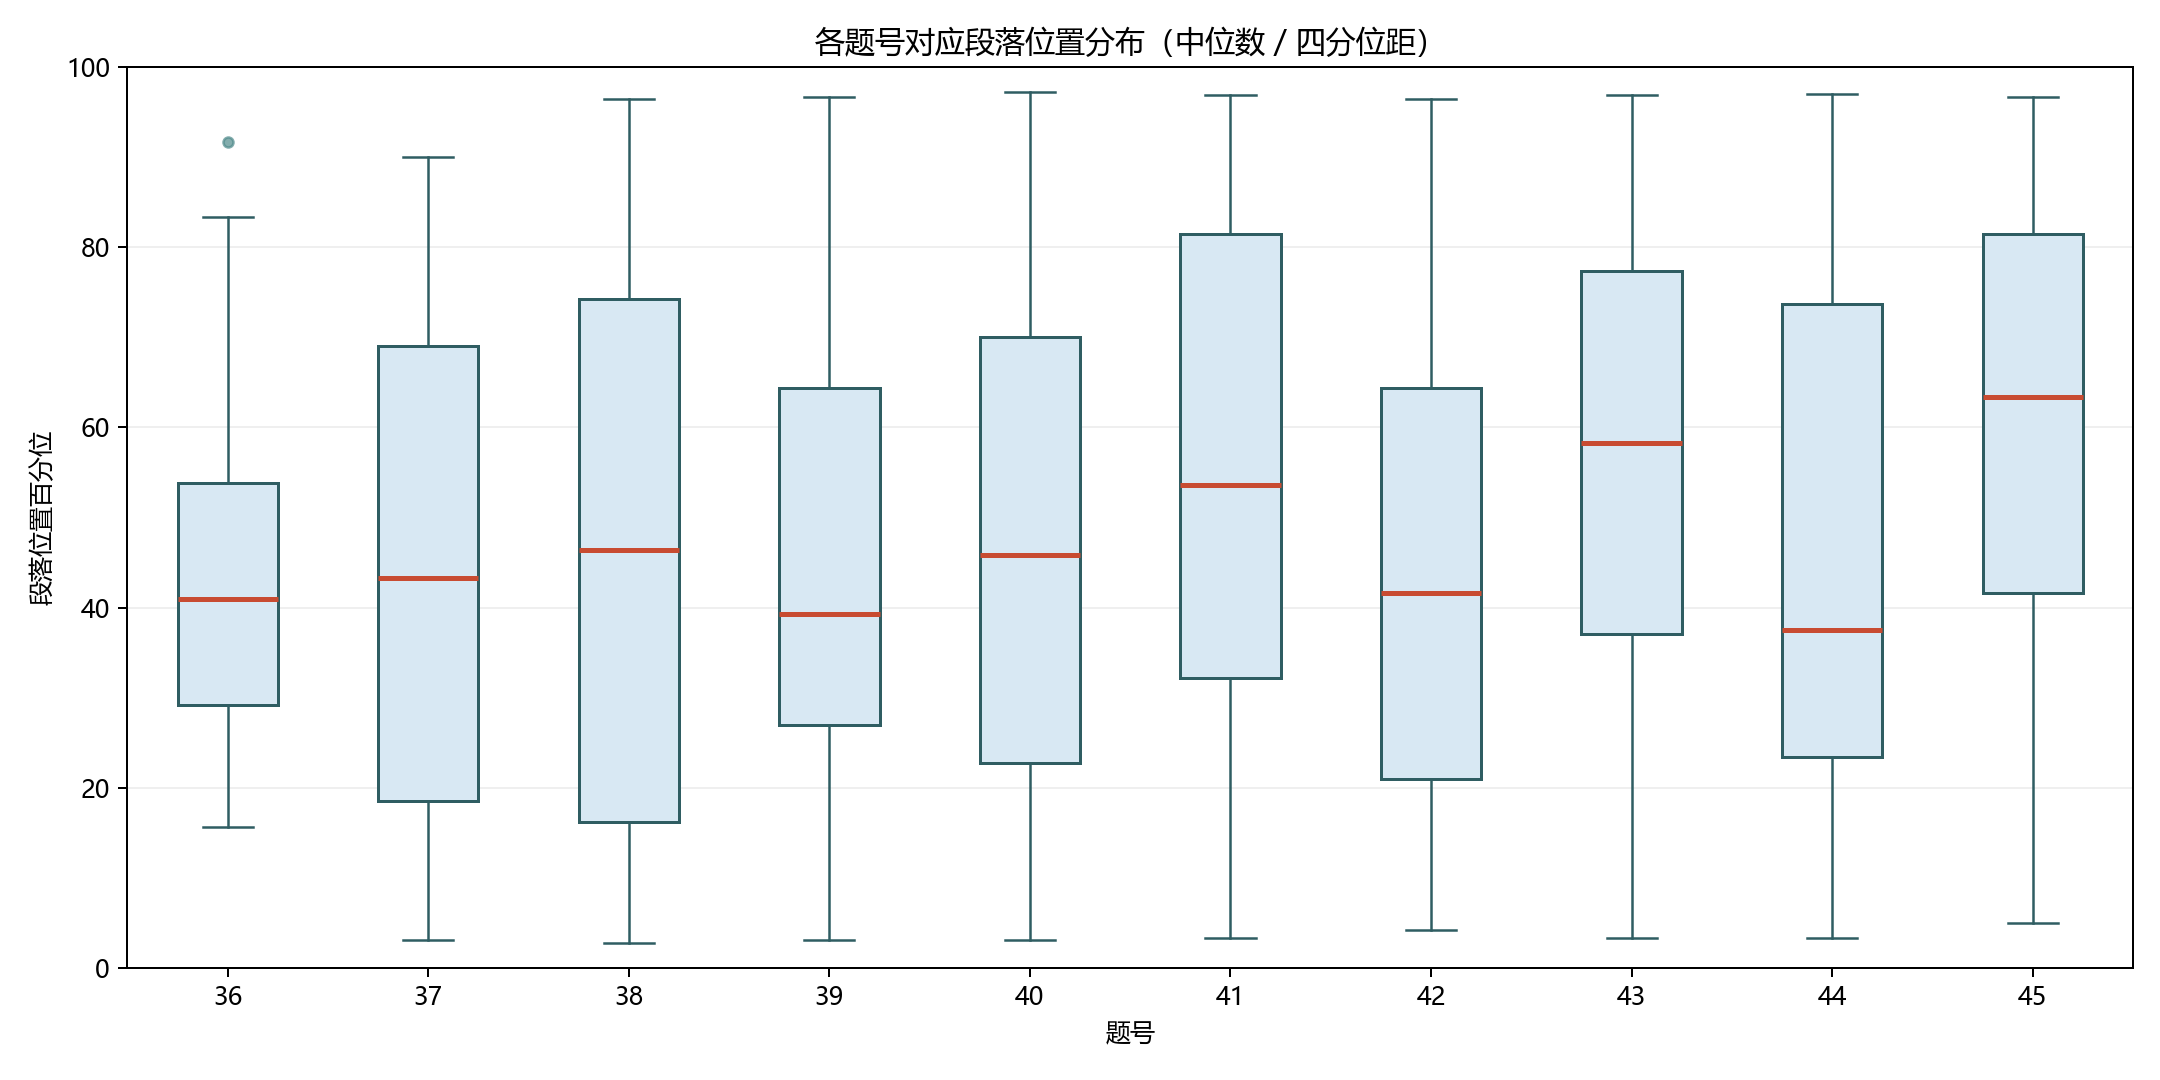
\includegraphics[width=0.92\linewidth]{question_position_boxplot.png}
\caption{question\_position\_boxplot.png}
\end{figure}


看什么：


\begin{itemize}
\item 中位数
\item 四分位距
\item 是否有长尾
\end{itemize}


适合干什么：


\begin{itemize}
\item 判断某题整体偏前偏后
\item 判断某题稳不稳
\end{itemize}


不适合干什么：


\begin{itemize}
\item 直接拿中位数押具体段落
\end{itemize}


\phantomsection
\subsubsection*{\CodeInline{question\_position\_band\_distribution.png}}
\addcontentsline{toc}{subsubsection}{question\_position\_band\_distribution.png}
\begin{figure}[H]
\centering
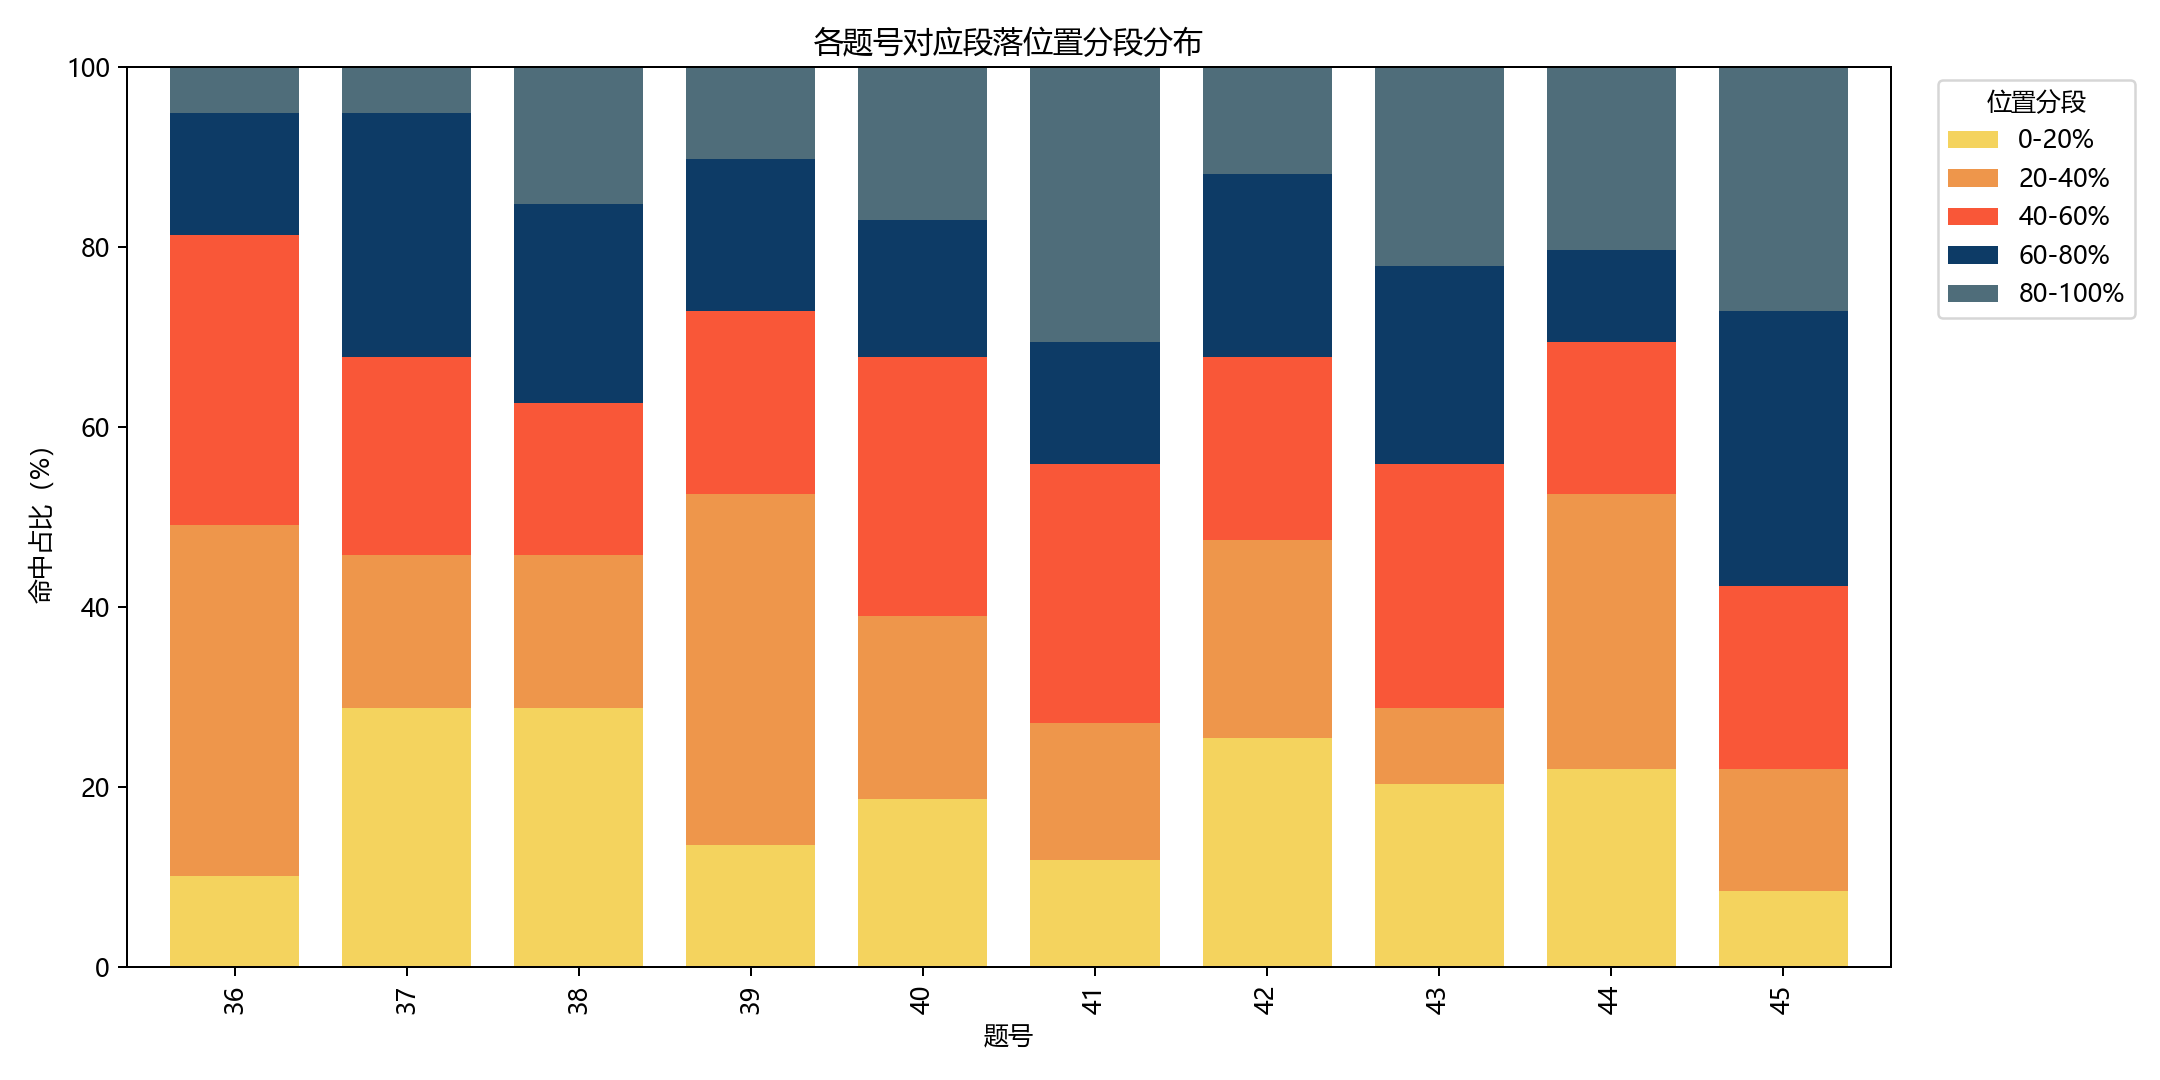
\includegraphics[width=0.92\linewidth]{question_position_band_distribution.png}
\caption{question\_position\_band\_distribution.png}
\end{figure}


看什么：


\begin{itemize}
\item 五个 20\% 大带的占比
\end{itemize}


适合干什么：


\begin{itemize}
\item 粗定位
\item 判断大区间主战区
\end{itemize}


不适合干什么：


\begin{itemize}
\item 精确定位到小段落
\end{itemize}


\phantomsection
\subsubsection*{\CodeInline{question\_position\_band\_heatmap.png}}
\addcontentsline{toc}{subsubsection}{question\_position\_band\_heatmap.png}
\begin{figure}[H]
\centering
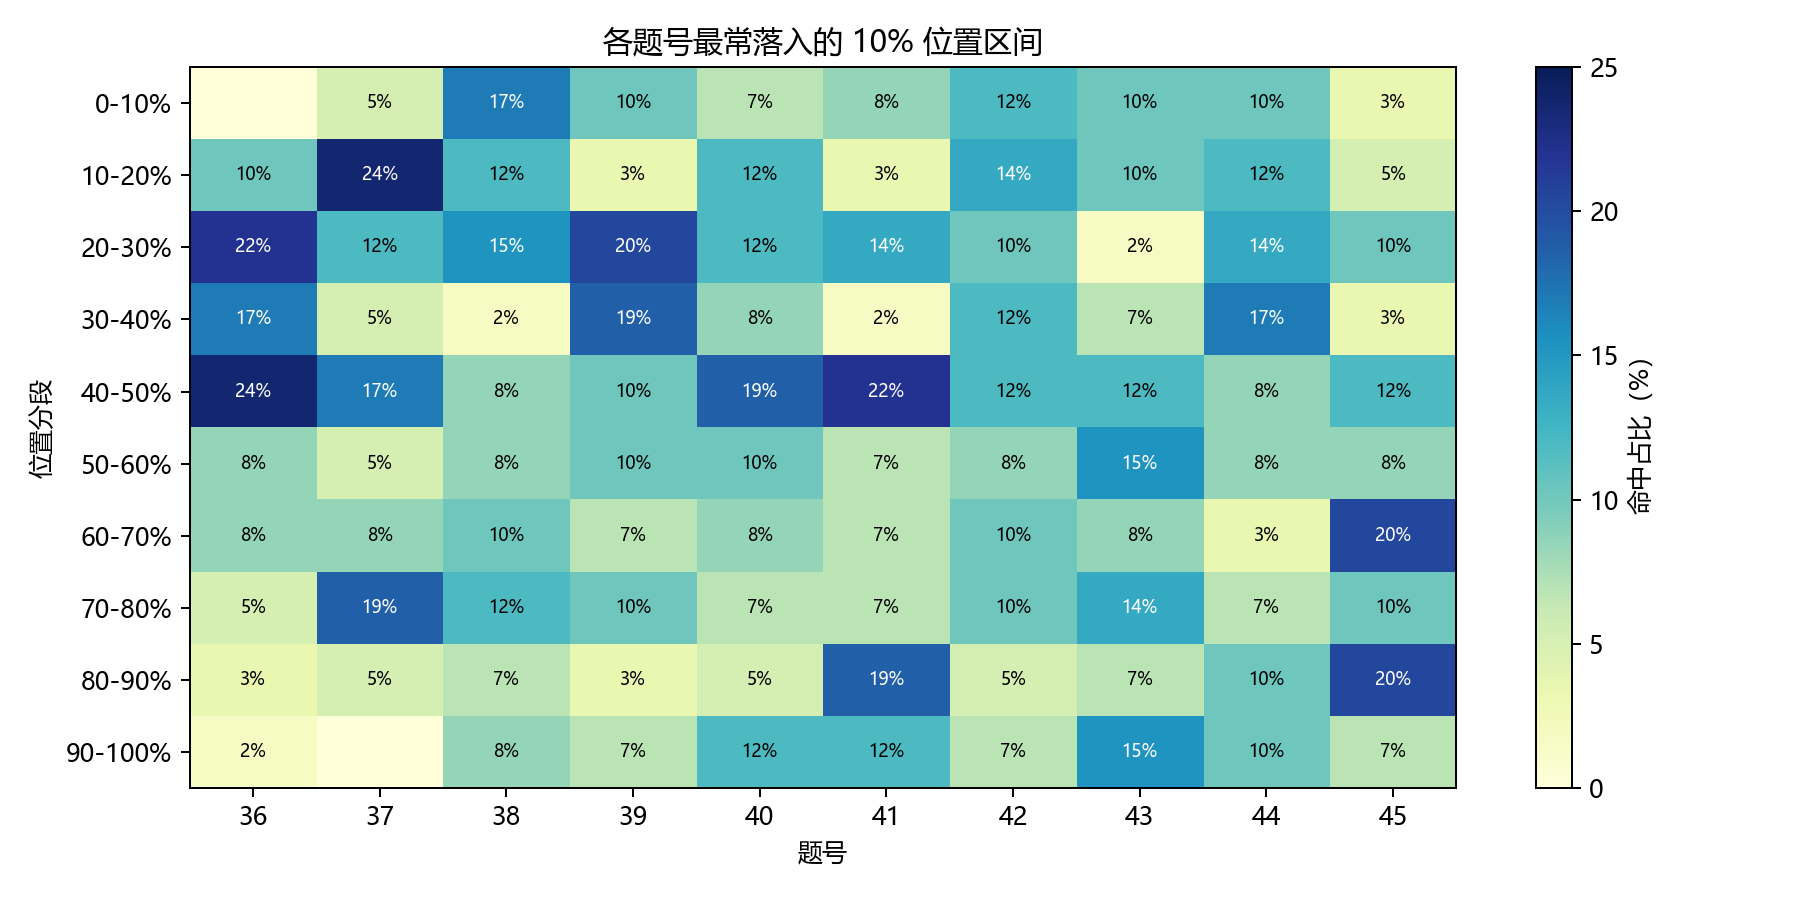
\includegraphics[width=0.92\linewidth]{question_position_band_heatmap.png}
\caption{question\_position\_band\_heatmap.png}
\end{figure}


看什么：


\begin{itemize}
\item 每个题在 10\% 热区上的高发位置
\end{itemize}


适合干什么：


\begin{itemize}
\item 看双峰结构
\item 看热区是否集中
\end{itemize}


\phantomsection
\subsubsection*{\CodeInline{question\_answer\_distribution.png}}
\addcontentsline{toc}{subsubsection}{question\_answer\_distribution.png}
\begin{figure}[H]
\centering
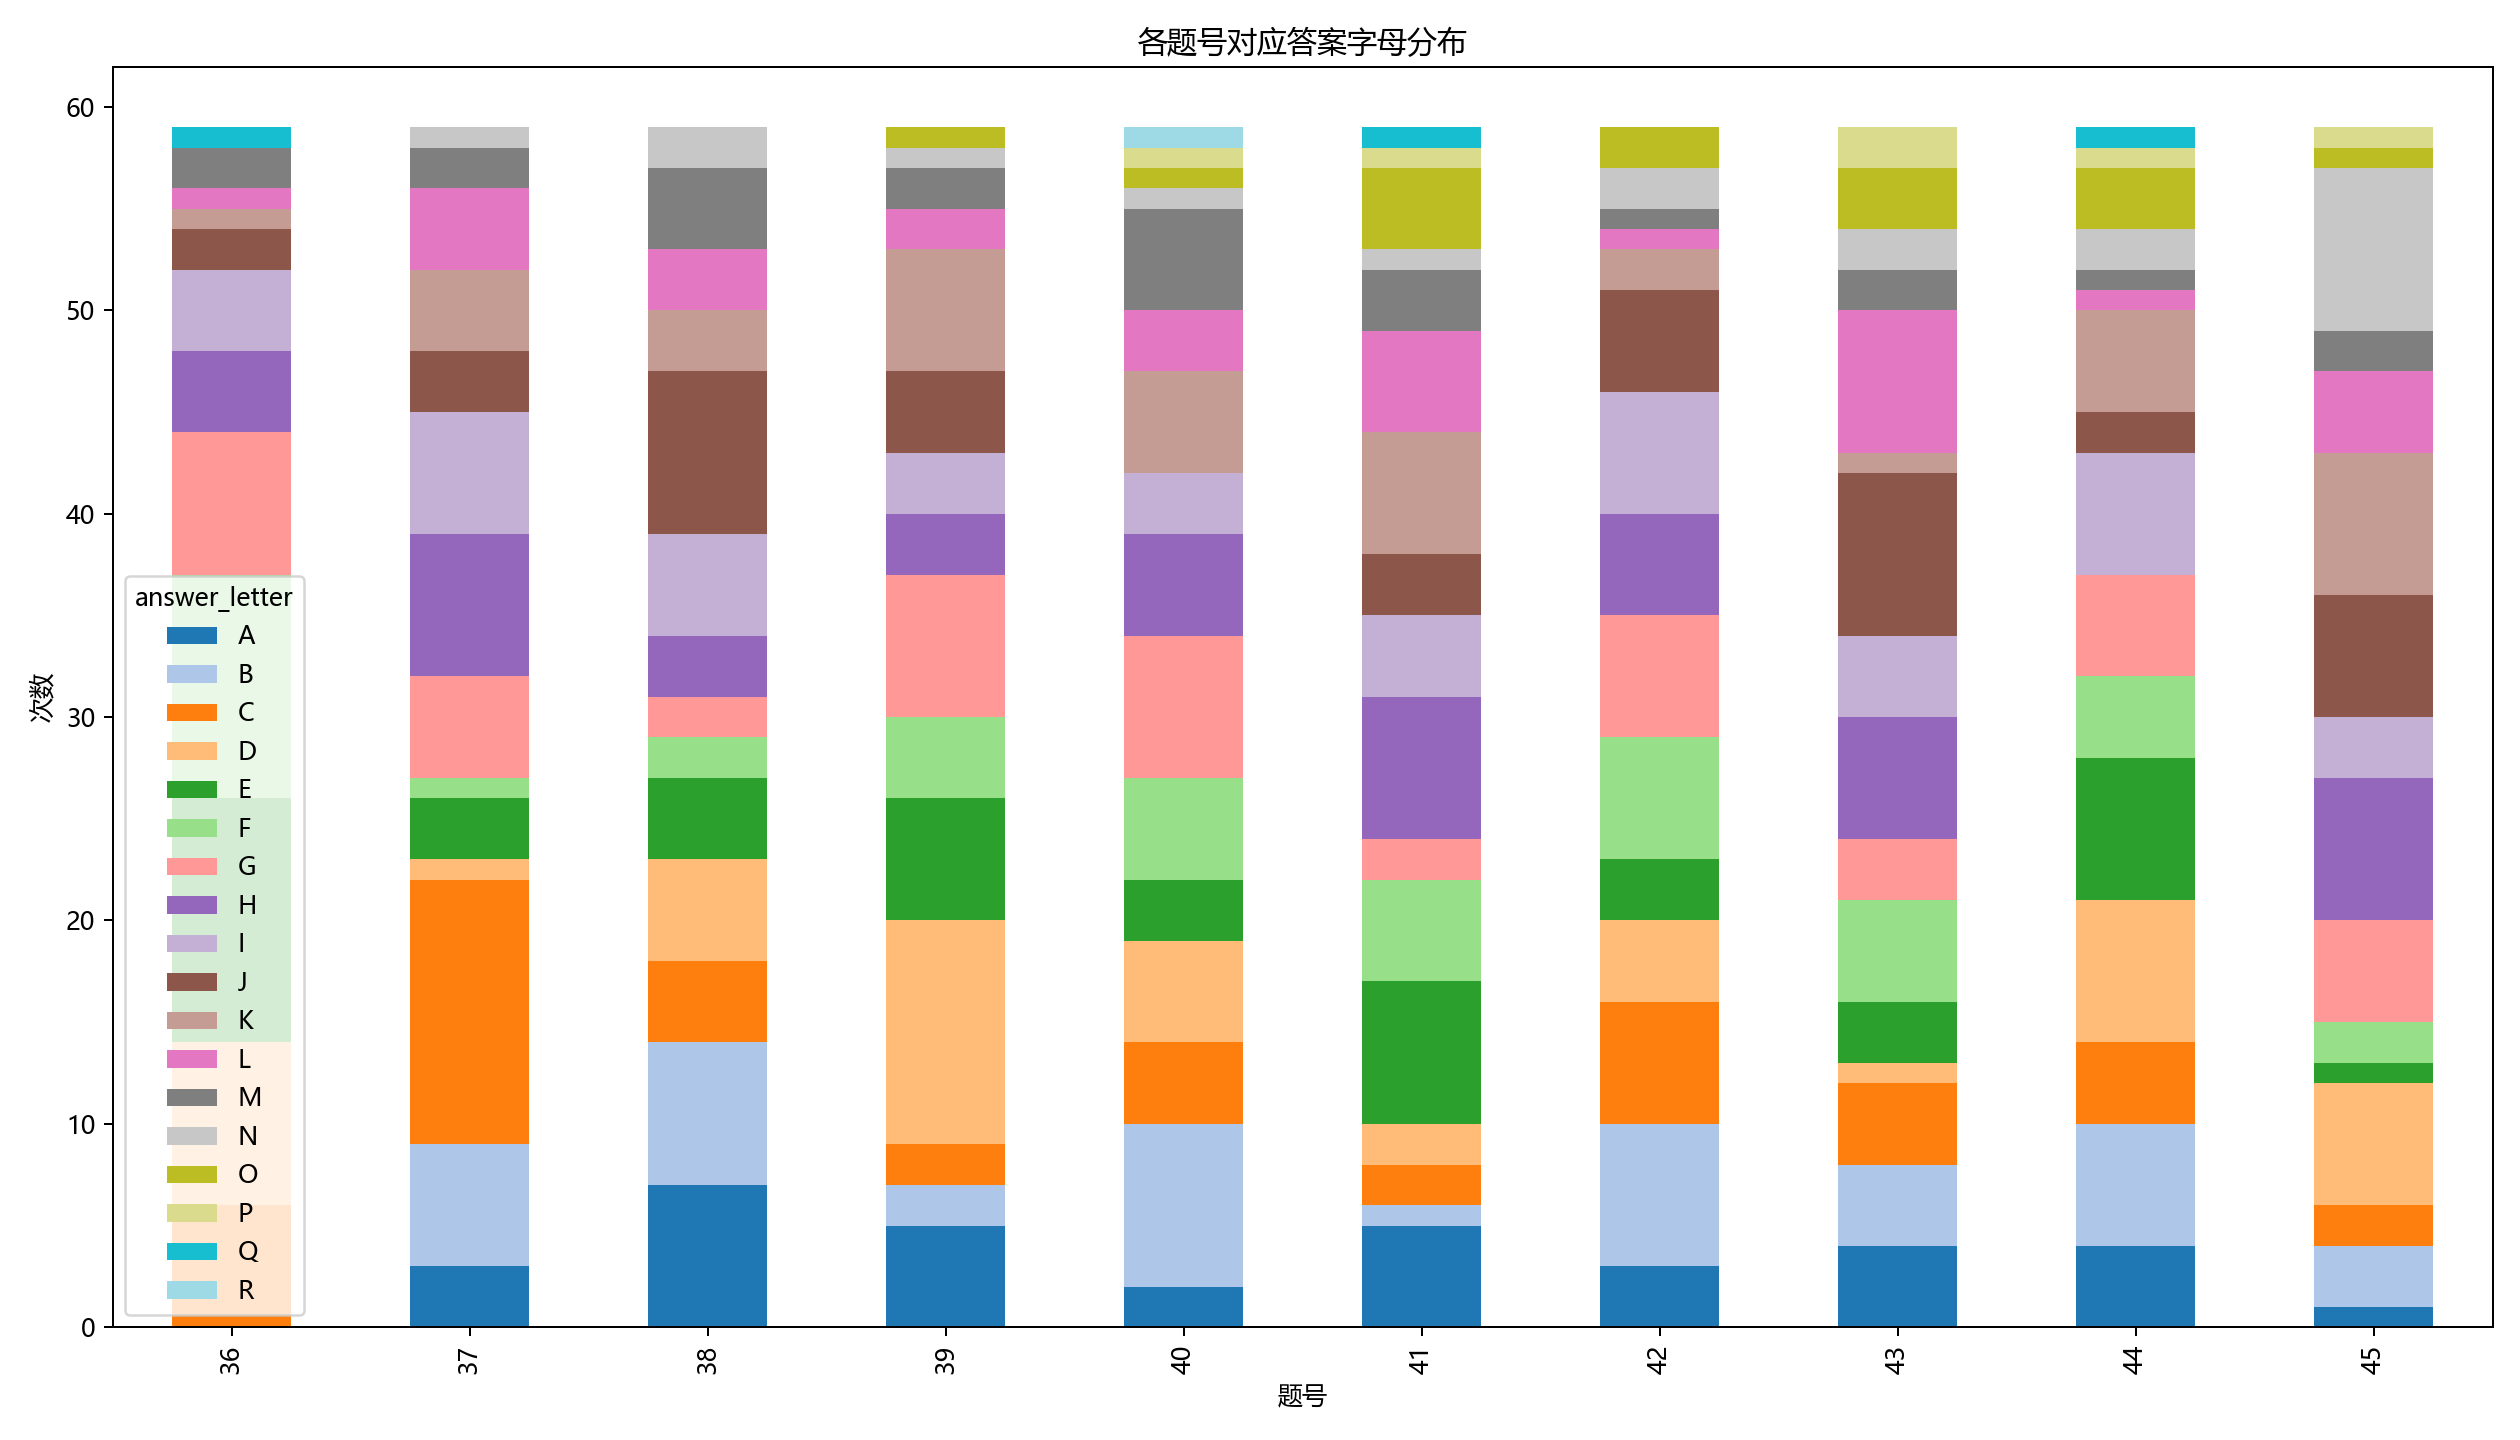
\includegraphics[width=0.92\linewidth]{question_answer_distribution.png}
\caption{question\_answer\_distribution.png}
\end{figure}


看什么：


\begin{itemize}
\item 每题最常对应哪些原文段落字母
\end{itemize}


适合干什么：


\begin{itemize}
\item 判断前段题、后段题倾向
\end{itemize}


不适合干什么：


\begin{itemize}
\item 直接押具体字母
\end{itemize}


\phantomsection
\subsubsection*{\CodeInline{letter\_to\_question\_heatmap.png}}
\addcontentsline{toc}{subsubsection}{letter\_to\_question\_heatmap.png}
\begin{figure}[H]
\centering
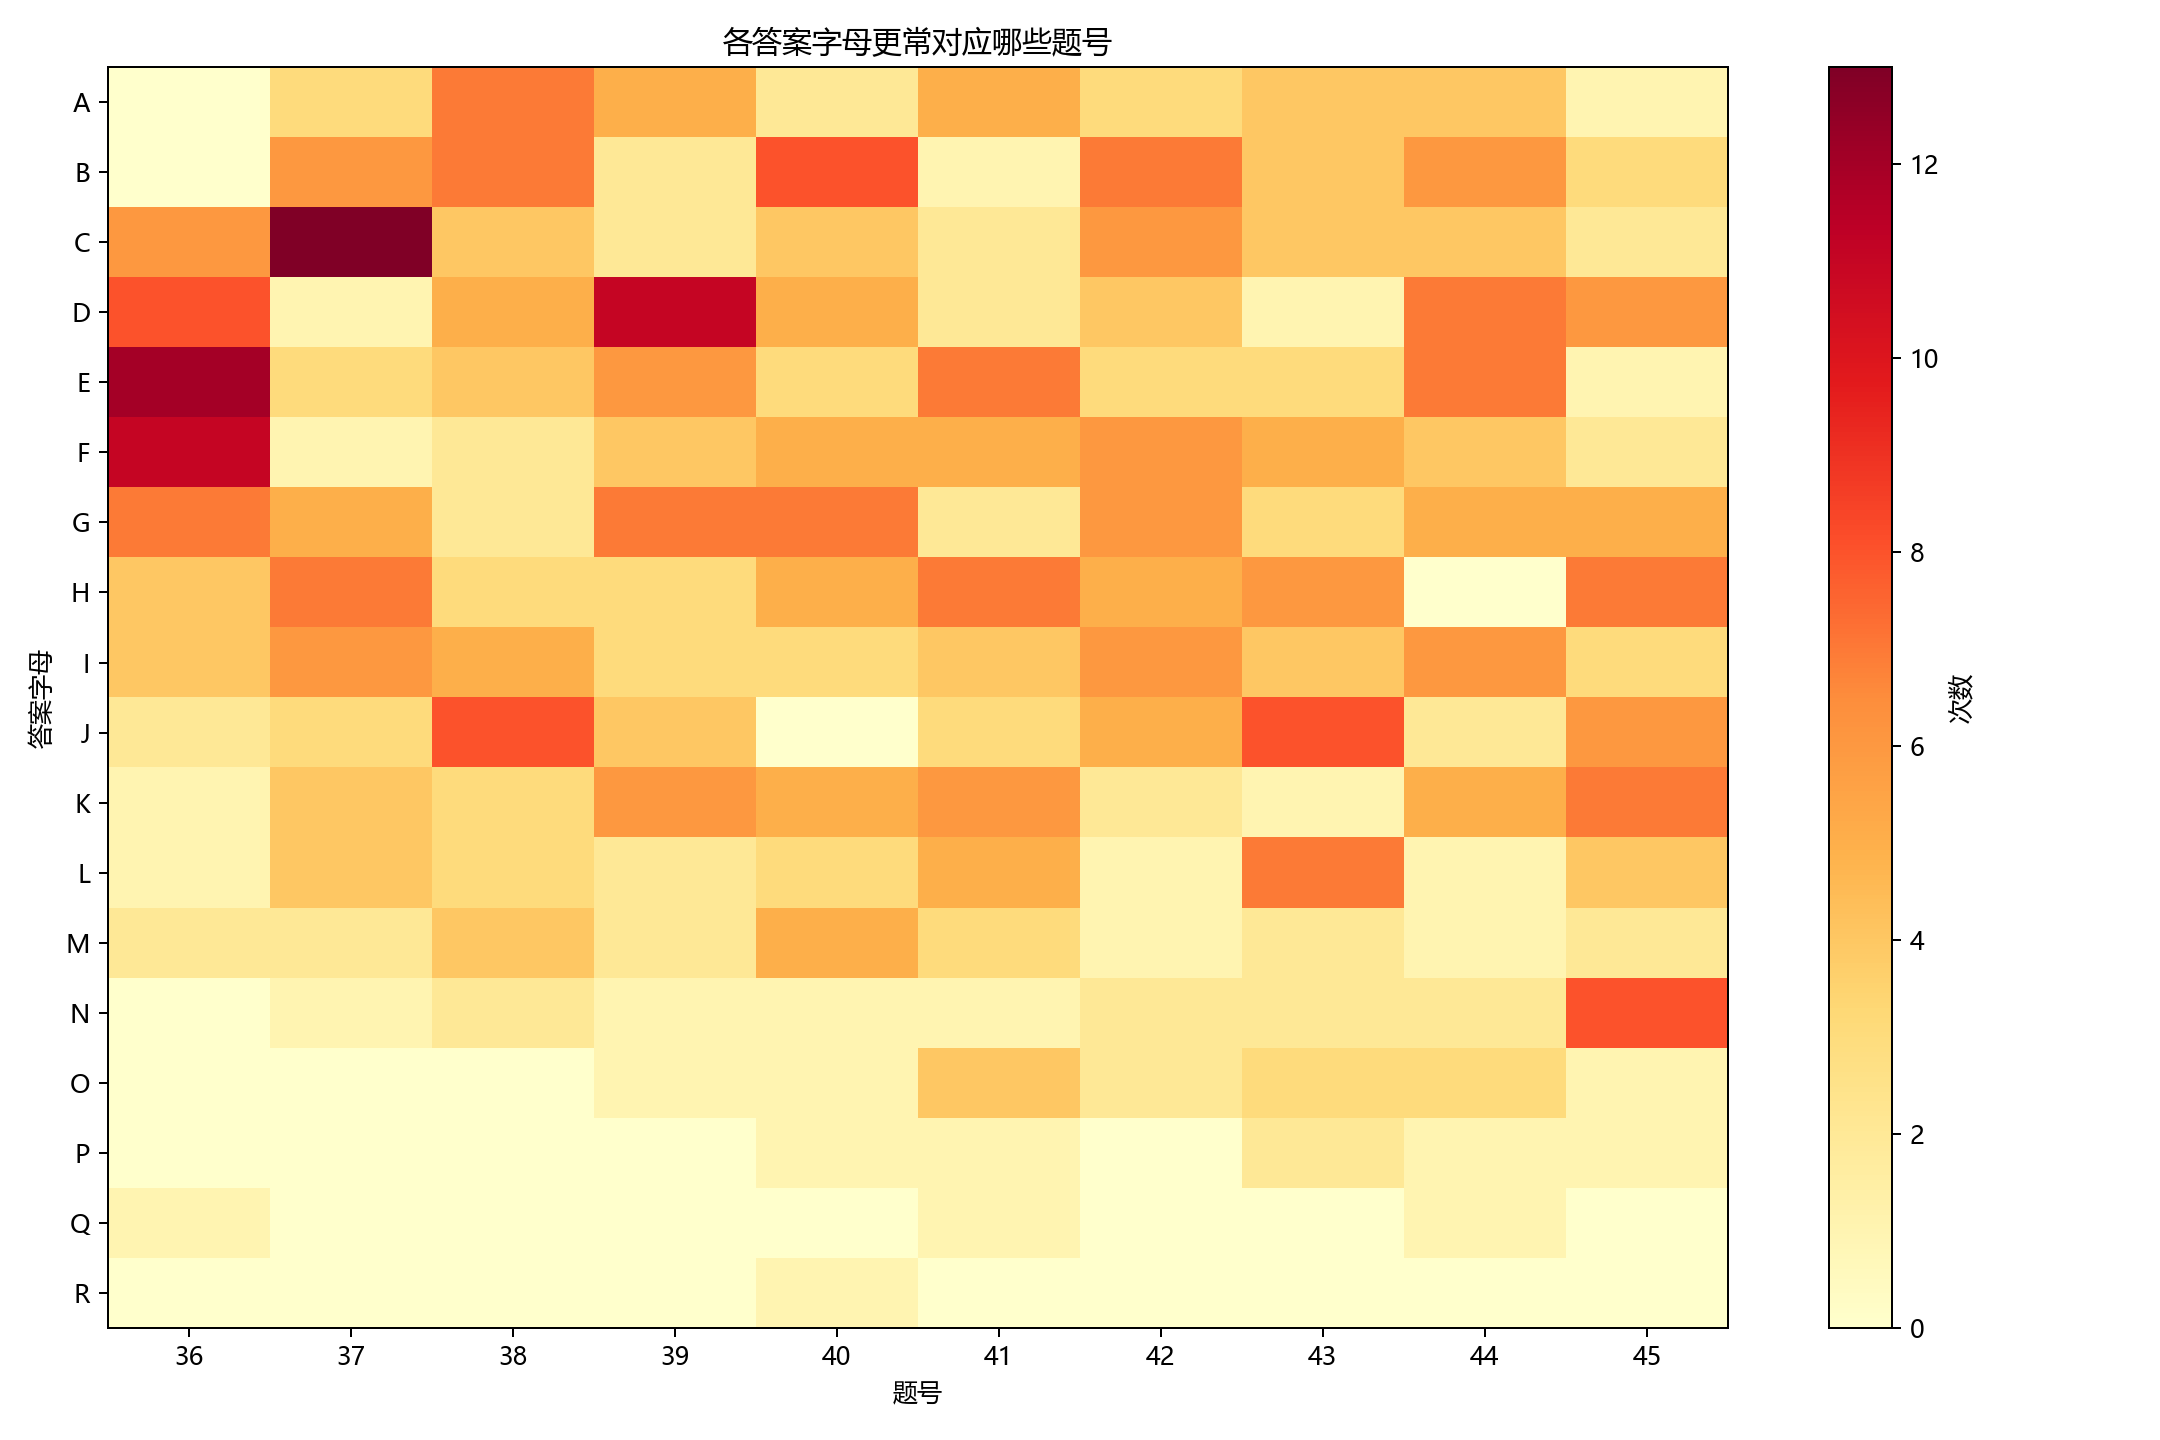
\includegraphics[width=0.92\linewidth]{letter_to_question_heatmap.png}
\caption{letter\_to\_question\_heatmap.png}
\end{figure}


看什么：


\begin{itemize}
\item 每个字母更偏向哪些题号
\end{itemize}


适合干什么：


\begin{itemize}
\item 后期排除
\end{itemize}


不适合干什么：


\begin{itemize}
\item 前期单独判断答案
\end{itemize}


一句话总结：


\textbf{图表最大的价值是粗筛、排除和辅助联动，不是单独定点。}


\phantomsection
\subsection*{3.4 图表文件索引}
\addcontentsline{toc}{subsection}{3.4 图表文件索引}


当前正文直接对应的图表文件均位于 \CodeInline{cet 6/\_analysis\_output/}：


\begin{itemize}
\item \CodeInline{question\_position\_boxplot.png}：单题位置箱线图，用来看中位数、四分位距与离散度。
\item \CodeInline{question\_position\_band\_distribution.png}：单题在五个 \CodeInline{20\%} 大带上的分布图，用来做粗定位。
\item \CodeInline{question\_position\_band\_heatmap.png}：单题在 \CodeInline{10\%} 细带上的热区图，用来观察双峰、散峰和局部集中。
\item \CodeInline{question\_position\_curve.png}：单题位置曲线图，用来辅助观察整体形态、长尾与多峰倾向。
\item \CodeInline{question\_answer\_distribution.png}：题号到原文段落字母的分布图，用来做后期排除与偏向判断。
\item \CodeInline{letter\_to\_question\_heatmap.png}：字母反向映射到题号的热力图，用来辅助判断某字母更常落在哪些题号上。
\end{itemize}


\phantomsection
\section*{4. 单题位置分布：先把基础层讲清楚}
\addcontentsline{toc}{section}{4. 单题位置分布：先把基础层讲清楚}


\phantomsection
\subsection*{4.1 粗粒度 20\% 分带分布}
\addcontentsline{toc}{subsection}{4.1 粗粒度 20\% 分带分布}


根据 \CodeInline{question\_position\_stats.csv}：


\begin{center}
\small
\setlength{\tabcolsep}{4pt}
\begin{longtable}{@{}>{\raggedright\arraybackslash}p{0.172\linewidth}>{\raggedright\arraybackslash}p{0.172\linewidth}>{\raggedright\arraybackslash}p{0.172\linewidth}>{\raggedright\arraybackslash}p{0.172\linewidth}>{\raggedright\arraybackslash}p{0.172\linewidth}@{}}
\toprule
\textbf{题号} & \textbf{主导 20\% 带} & \textbf{占比} & \textbf{次主导 20\% 带} & \textbf{占比} \\
\midrule
\endfirsthead
\toprule
\textbf{题号} & \textbf{主导 20\% 带} & \textbf{占比} & \textbf{次主导 20\% 带} & \textbf{占比} \\
\midrule
\endhead
Q36 & \CodeInline{20-40\%} & 37.50\% & \CodeInline{40-60\%} & 33.93\% \\
Q37 & \CodeInline{0-20\%} & 30.36\% & \CodeInline{60-80\%} & 26.79\% \\
Q38 & \CodeInline{0-20\%} & 26.79\% & \CodeInline{60-80\%} & 23.21\% \\
Q39 & \CodeInline{20-40\%} & 39.29\% & \CodeInline{40-60\%} & 21.43\% \\
Q40 & \CodeInline{40-60\%} & 28.57\% & \CodeInline{20-40\%} & 21.43\% \\
Q41 & \CodeInline{80-100\%} & 32.14\% & \CodeInline{40-60\%} & 28.57\% \\
Q42 & \CodeInline{0-20\%} & 26.79\% & \CodeInline{20-40\%} & 21.43\% \\
Q43 & \CodeInline{40-60\%} & 28.57\% & \CodeInline{0-20\%} & 21.43\% \\
Q44 & \CodeInline{20-40\%} & 30.36\% & \CodeInline{0-20\%} & 21.43\% \\
Q45 & \CodeInline{60-80\%} & 32.14\% & \CodeInline{80-100\%} & 23.21\% \\
\bottomrule
\end{longtable}
\normalsize
\end{center}


可以先得到最基础的单题印象：


\begin{itemize}
\item \CodeInline{Q36 / Q39 / Q44} 偏前中段
\item \CodeInline{Q41 / Q45} 偏后段
\item \CodeInline{Q38 / Q42 / Q43} 分散度更高
\end{itemize}


\phantomsection
\subsection*{4.2 细粒度 10\% 热区分布}
\addcontentsline{toc}{subsection}{4.2 细粒度 10\% 热区分布}


根据 \CodeInline{question\_position\_fine\_stats.csv}：


\begin{center}
\small
\setlength{\tabcolsep}{4pt}
\begin{longtable}{@{}>{\raggedright\arraybackslash}p{0.172\linewidth}>{\raggedright\arraybackslash}p{0.172\linewidth}>{\raggedright\arraybackslash}p{0.172\linewidth}>{\raggedright\arraybackslash}p{0.172\linewidth}>{\raggedright\arraybackslash}p{0.172\linewidth}@{}}
\toprule
\textbf{题号} & \textbf{主导 10\% 带} & \textbf{占比} & \textbf{次主导 10\% 带} & \textbf{占比} \\
\midrule
\endfirsthead
\toprule
\textbf{题号} & \textbf{主导 10\% 带} & \textbf{占比} & \textbf{次主导 10\% 带} & \textbf{占比} \\
\midrule
\endhead
Q36 & \CodeInline{40-50\%} & 25.00\% & \CodeInline{20-30\%} & 19.64\% \\
Q37 & \CodeInline{10-20\%} & 25.00\% & \CodeInline{70-80\%} & 17.86\% \\
Q38 & \CodeInline{20-30\%} & 16.07\% & \CodeInline{0-10\%} & 14.29\% \\
Q39 & \CodeInline{20-30\%} & 21.43\% & \CodeInline{30-40\%} & 17.86\% \\
Q40 & \CodeInline{40-50\%} & 19.64\% & \CodeInline{20-30\%} & 12.50\% \\
Q41 & \CodeInline{40-50\%} & 21.43\% & \CodeInline{80-90\%} & 19.64\% \\
Q42 & \CodeInline{10-20\%} & 14.29\% & \CodeInline{0-10\%} & 12.50\% \\
Q43 & \CodeInline{50-60\%} & 16.07\% & \CodeInline{70-80\%} & 14.29\% \\
Q44 & \CodeInline{30-40\%} & 17.86\% & \CodeInline{20-30\%} & 12.50\% \\
Q45 & \CodeInline{60-70\%} & 21.43\% & \CodeInline{80-90\%} & 17.86\% \\
\bottomrule
\end{longtable}
\normalsize
\end{center}


观察重点：


\begin{itemize}
\item \CodeInline{Q37} 的双峰很明显：既可能靠前，也可能很靠后
\item \CodeInline{Q41} 也存在中后双峰
\item \CodeInline{Q45} 的高频热区主要集中在后段
\item \CodeInline{Q38 / Q42 / Q43 / Q44} 的主峰都不够尖
\end{itemize}


\phantomsection
\subsection*{4.3 分散度指标说明}
\addcontentsline{toc}{subsection}{4.3 分散度指标说明}


\CodeInline{band\_entropy\_20} 和 \CodeInline{band\_entropy\_10} 越高，说明该题越分散。


典型值：


\begin{itemize}
\item \CodeInline{Q38}: \CodeInline{band\_entropy\_20 = 0.9849},\allowbreak{} \CodeInline{band\_entropy\_10 = 0.9603}
\item \CodeInline{Q42}: \CodeInline{band\_entropy\_20 = 0.9768},\allowbreak{} \CodeInline{band\_entropy\_10 = 0.9792}
\item \CodeInline{Q44}: \CodeInline{band\_entropy\_20 = 0.9663},\allowbreak{} \CodeInline{band\_entropy\_10 = 0.9713}
\end{itemize}


这些题都说明：


\begin{itemize}
\item 无条件时不够稳定
\item 更适合条件化处理
\end{itemize}


相对更稳的题：


\begin{itemize}
\item \CodeInline{Q36}: \CodeInline{band\_entropy\_20 = 0.8606}
\end{itemize}


这也解释了为什么：


\begin{itemize}
\item \CodeInline{Q36} 适合定区
\item \CodeInline{Q38 / Q42 / Q43} 更适合条件做题
\end{itemize}


\phantomsection
\subsection*{4.4 单题连续窗口覆盖率}
\addcontentsline{toc}{subsection}{4.4 单题连续窗口覆盖率}


根据 \CodeInline{question\_strategy\_features.csv}：


\begin{itemize}
\item \CodeInline{Q36} 的最佳连续 40\% 窗口是 \CodeInline{20-60\%}，覆盖 \CodeInline{71.43\%}
\item \CodeInline{Q39} 的最佳连续 40\% 窗口是 \CodeInline{20-60\%}，覆盖 \CodeInline{60.71\%}
\item \CodeInline{Q41} 的最佳连续 40\% 窗口是 \CodeInline{60-100\%}，覆盖 \CodeInline{44.64\%}
\item \CodeInline{Q45} 的最佳连续 40\% 窗口是 \CodeInline{60-100\%}，覆盖 \CodeInline{55.36\%}
\end{itemize}


这个指标很重要，因为它直接对应“单题裸做时的最佳大区间”。


\phantomsection
\section*{5. 答案字母分布层面还能看到什么}
\addcontentsline{toc}{section}{5. 答案字母分布层面还能看到什么}


\phantomsection
\subsection*{5.1 单题对应字母分布}
\addcontentsline{toc}{subsection}{5.1 单题对应字母分布}


根据 \CodeInline{question\_answer\_summary.csv}：


\begin{itemize}
\item \CodeInline{Q36} 的高频字母是 \CodeInline{E}，占比 \CodeInline{20.34\%}
\item \CodeInline{Q37} 的高频字母是 \CodeInline{C}，占比 \CodeInline{22.03\%}
\item \CodeInline{Q41} 的前两高字母并列，\CodeInline{top\_gap\_pct = 0}
\item \CodeInline{Q44} 的前两高字母也并列，\CodeInline{top\_gap\_pct = 0}
\end{itemize}


这说明：


\begin{itemize}
\item 大多数题号的字母分布主峰并不尖
\item 靠字母本身押题的价值有限
\end{itemize}


\phantomsection
\subsection*{5.2 反向看：某字母更偏向哪些题号}
\addcontentsline{toc}{subsection}{5.2 反向看：某字母更偏向哪些题号}


根据 \CodeInline{letter\_to\_question\_summary.csv}：


\begin{itemize}
\item \CodeInline{N} 最常见于 \CodeInline{Q45}，占比 \CodeInline{40.0\%}
\item \CodeInline{C} 最常见于 \CodeInline{Q37}，占比 \CodeInline{27.66\%}
\item \CodeInline{E} 最常见于 \CodeInline{Q36}，占比 \CodeInline{24.49\%}
\item \CodeInline{F} 最常见于 \CodeInline{Q36}，占比 \CodeInline{24.44\%}
\end{itemize}


但整体看，大多数字母的 \CodeInline{reverse\_entropy} 仍不低， 说明：


\begin{itemize}
\item 字母更适合作为排除工具
\item 不适合作为主判断工具
\end{itemize}


\phantomsection
\subsection*{5.3 字母层面的结构性信息}
\addcontentsline{toc}{subsection}{5.3 字母层面的结构性信息}


继续看相邻题的字母距离：


根据 \CodeInline{adjacent\_question\_relation\_stats.csv}：


\begin{itemize}
\item \CodeInline{Q40/Q41} 的 \CodeInline{within\_2\_letters\_pct = 3.57\%}
\item \CodeInline{Q43/Q44} 的 \CodeInline{within\_2\_letters\_pct = 0\%}
\item \CodeInline{Q44/Q45} 的 \CodeInline{within\_2\_letters\_pct = 7.14\%}
\end{itemize}


这说明：


\begin{itemize}
\item 相邻题不仅段落位置常常不近
\item 连字母顺序上也经常分离
\end{itemize}


\phantomsection
\section*{6. 单题角色重估}
\addcontentsline{toc}{section}{6. 单题角色重估}


\phantomsection
\subsection*{6.1 \CodeInline{Q36}：位置锚，不是起手锚}
\addcontentsline{toc}{subsection}{6.1 Q36：位置锚，不是起手锚}


根据 \CodeInline{question\_order\_profile.csv}：


\begin{itemize}
\item \CodeInline{median\_rank = 5.0}
\item \CodeInline{mean\_rank = 4.96}
\item \CodeInline{earliest\_pct = 0\%}
\item \CodeInline{top2\_earliest\_pct = 8.93\%}
\end{itemize}


结论：


\begin{itemize}
\item 它不是典型最早出题
\item 但它的单题分布更稳
\item 所以它是位置锚，不是默认起手锚
\end{itemize}


\phantomsection
\subsection*{6.2 \CodeInline{Q37}：前段奇数锚}
\addcontentsline{toc}{subsection}{6.2 Q37：前段奇数锚}


\begin{itemize}
\item \CodeInline{earliest\_pct = 10.71\%}
\item \CodeInline{top2\_earliest\_pct = 30.36\%}
\item \CodeInline{top3\_earliest\_pct = 44.64\%}
\end{itemize}


结论：


\begin{itemize}
\item 前段扫描时，它比 \CodeInline{Q36} 更像会先露头的题
\end{itemize}


\phantomsection
\subsection*{6.3 \CodeInline{Q38}：摆动题、反推题}
\addcontentsline{toc}{subsection}{6.3 Q38：摆动题、反推题}


\begin{itemize}
\item \CodeInline{earliest\_pct = 19.64\%}
\item \CodeInline{top2\_latest\_pct = 19.64\%}
\item \CodeInline{median\_rank = 5.5}
\end{itemize}


结论：


\begin{itemize}
\item 位置摆动大
\item 不适合裸做
\item 但适合做出后立刻反推别题
\end{itemize}


\phantomsection
\subsection*{6.4 \CodeInline{Q41} 与 \CodeInline{Q45}：后段双锚}
\addcontentsline{toc}{subsection}{6.4 Q41 与 Q45：后段双锚}


\CodeInline{Q41}：


\begin{itemize}
\item \CodeInline{top2\_latest\_pct = 33.93\%}
\end{itemize}


\CodeInline{Q45}：


\begin{itemize}
\item \CodeInline{top3\_latest\_pct = 44.64\%}
\end{itemize}


结论：


\begin{itemize}
\item \CodeInline{Q41} 更像真正的后段终点锚
\item \CodeInline{Q45} 是强后段锚，但不是唯一尾题
\end{itemize}


\phantomsection
\subsection*{6.5 \CodeInline{Q44}：中后段总枢纽}
\addcontentsline{toc}{subsection}{6.5 Q44：中后段总枢纽}


\begin{itemize}
\item \CodeInline{median\_rank = 4.0}
\item \CodeInline{rule\_count\_gain10 = 24}
\item \CodeInline{rule\_count\_gain15 = 16}
\end{itemize}


结论：


\begin{itemize}
\item 它自己不一定最晚出现
\item 但它是最强的条件源题
\end{itemize}


\phantomsection
\section*{7. 题间无条件相关性：先看整体结构}
\addcontentsline{toc}{section}{7. 题间无条件相关性：先看整体结构}


\phantomsection
\subsection*{7.1 相邻题通常不是就近题}
\addcontentsline{toc}{subsection}{7.1 相邻题通常不是就近题}


根据 \CodeInline{question\_pair\_relation\_stats.csv} 与 \CodeInline{adjacent\_question\_relation\_stats.csv}：


\phantomsection
\subsubsection*{\CodeInline{Q40/Q41}}
\addcontentsline{toc}{subsubsection}{Q40/Q41}


\begin{itemize}
\item \CodeInline{spearman\_pct = -0.2106}
\item \CodeInline{within\_2\_paragraph\_pct = 3.57\%}
\item \CodeInline{median\_gap\_paragraphs = 4.0}
\end{itemize}


\phantomsection
\subsubsection*{\CodeInline{Q41/Q42}}
\addcontentsline{toc}{subsubsection}{Q41/Q42}


\begin{itemize}
\item \CodeInline{spearman\_pct = -0.3831}
\item \CodeInline{within\_2\_paragraph\_pct = 8.93\%}
\item \CodeInline{median\_gap\_paragraphs = -4.0}
\end{itemize}


\phantomsection
\subsubsection*{\CodeInline{Q43/Q44}}
\addcontentsline{toc}{subsubsection}{Q43/Q44}


\begin{itemize}
\item \CodeInline{spearman\_pct = -0.4364}
\item \CodeInline{within\_2\_paragraph\_pct = 0\%}
\item \CodeInline{median\_gap\_paragraphs = -4.0}
\end{itemize}


\phantomsection
\subsubsection*{\CodeInline{Q44/Q45}}
\addcontentsline{toc}{subsubsection}{Q44/Q45}


\begin{itemize}
\item \CodeInline{spearman\_pct = -0.5107}
\item \CodeInline{within\_2\_paragraph\_pct = 7.14\%}
\item \CodeInline{median\_gap\_paragraphs = 3.5}
\end{itemize}


结论：


\begin{itemize}
\item 相邻题不但不常相邻
\item 往往还存在明显错位
\end{itemize}


\phantomsection
\subsection*{7.2 隔一题的同奇偶链更强}
\addcontentsline{toc}{subsection}{7.2 隔一题的同奇偶链更强}


\phantomsection
\subsubsection*{\CodeInline{Q37/Q39}}
\addcontentsline{toc}{subsubsection}{Q37/Q39}


\begin{itemize}
\item \CodeInline{spearman\_pct = 0.2981}
\item \CodeInline{within\_2\_paragraph\_pct = 51.79\%}
\item \CodeInline{same\_half\_pct = 60.71\%}
\item \CodeInline{median\_gap\_paragraphs = 1.0}
\end{itemize}


\phantomsection
\subsubsection*{\CodeInline{Q36/Q38}}
\addcontentsline{toc}{subsubsection}{Q36/Q38}


\begin{itemize}
\item \CodeInline{spearman\_pct = 0.2863}
\item \CodeInline{within\_2\_paragraph\_pct = 41.07\%}
\item \CodeInline{same\_half\_pct = 53.57\%}
\item \CodeInline{median\_gap\_paragraphs = 1.0}
\end{itemize}


\phantomsection
\subsubsection*{\CodeInline{Q43/Q45}}
\addcontentsline{toc}{subsubsection}{Q43/Q45}


\begin{itemize}
\item \CodeInline{spearman\_pct = 0.2078}
\item \CodeInline{within\_2\_paragraph\_pct = 41.07\%}
\item \CodeInline{same\_half\_pct = 67.86\%}
\item \CodeInline{median\_gap\_paragraphs = 1.0}
\end{itemize}


结论：


\begin{itemize}
\item 真正值得联动的是隔一题的同奇偶链
\item 不是相邻题
\end{itemize}


\phantomsection
\subsection*{7.3 字母层面也支持“相邻题分离，隔一题更近”}
\addcontentsline{toc}{subsection}{7.3 字母层面也支持“相邻题分离，隔一题更近”}


根据 \CodeInline{adjacent\_question\_relation\_stats.csv} 和补充复核：


\begin{itemize}
\item 相邻题字母差绝对值 \CodeInline{<= 2} 的比例整体只有 \CodeInline{7.14\%}
\item 隔一题字母差绝对值 \CodeInline{<= 2} 的比例达到 \CodeInline{42.19\%}
\end{itemize}


所以：


\begin{itemize}
\item 相邻题不仅段落不近
\item 字母顺序上也经常分离
\end{itemize}


\phantomsection
\section*{8. 条件联动：这轮最有价值的新信息}
\addcontentsline{toc}{section}{8. 条件联动：这轮最有价值的新信息}


\phantomsection
\subsection*{8.1 最强跳带规则}
\addcontentsline{toc}{subsection}{8.1 最强跳带规则}


\phantomsection
\subsubsection*{规则 A：\CodeInline{Q39 = 0-20\% -> Q41 = 60-100\%}}
\addcontentsline{toc}{subsubsection}{规则 A：Q39 = 0-20\% -> Q41 = 60-100\%}


\begin{itemize}
\item \CodeInline{support\_count = 8}
\item \CodeInline{target\_best\_40\_window = 60-100\%}
\item \CodeInline{target\_best\_40\_coverage\_pct = 100.0\%}
\item \CodeInline{gain\_40\_pct = +55.36}
\end{itemize}


\phantomsection
\subsubsection*{规则 B：\CodeInline{Q44 = 0-20\% -> Q45 = 60-100\%}}
\addcontentsline{toc}{subsubsection}{规则 B：Q44 = 0-20\% -> Q45 = 60-100\%}


\begin{itemize}
\item \CodeInline{support\_count = 12}
\item \CodeInline{target\_best\_40\_window = 60-100\%}
\item \CodeInline{target\_best\_40\_coverage\_pct = 91.67\%}
\item \CodeInline{gain\_40\_pct = +32.74}
\end{itemize}


\phantomsection
\subsection*{8.2 最强压缩窗口规则}
\addcontentsline{toc}{subsection}{8.2 最强压缩窗口规则}


\phantomsection
\subsubsection*{规则 C：\CodeInline{Q37 = 0-20\% -> Q39 = 10-50\%}}
\addcontentsline{toc}{subsubsection}{规则 C：Q37 = 0-20\% -> Q39 = 10-50\%}


\begin{itemize}
\item \CodeInline{support\_count = 17}
\item \CodeInline{target\_best\_40\_coverage\_pct = 88.24\%}
\item \CodeInline{gain\_40\_pct = +27.53}
\end{itemize}


\phantomsection
\subsubsection*{规则 D：\CodeInline{Q42 = 20-40\% -> Q44 = 0-40\%}}
\addcontentsline{toc}{subsubsection}{规则 D：Q42 = 20-40\% -> Q44 = 0-40\%}


\begin{itemize}
\item \CodeInline{support\_count = 12}
\item \CodeInline{target\_best\_40\_coverage\_pct = 91.67\%}
\item \CodeInline{gain\_40\_pct = +39.88}
\end{itemize}


\phantomsection
\subsubsection*{规则 E：\CodeInline{Q42 = 20-40\% -> Q45 = 50-90\%}}
\addcontentsline{toc}{subsubsection}{规则 E：Q42 = 20-40\% -> Q45 = 50-90\%}


\begin{itemize}
\item \CodeInline{support\_count = 12}
\item \CodeInline{target\_best\_40\_coverage\_pct = 91.67\%}
\item \CodeInline{gain\_40\_pct = +32.74}
\end{itemize}


\phantomsection
\subsection*{8.3 最强反向排除规则}
\addcontentsline{toc}{subsection}{8.3 最强反向排除规则}


\phantomsection
\subsubsection*{规则 F：\CodeInline{Q41 = 80-100\% -> Q40 = 20-60\%}}
\addcontentsline{toc}{subsubsection}{规则 F：Q41 = 80-100\% -> Q40 = 20-60\%}


\begin{itemize}
\item \CodeInline{support\_count = 18}
\item \CodeInline{target\_best\_40\_coverage\_pct = 88.89\%}
\item \CodeInline{gain\_40\_pct = +37.10}
\end{itemize}


\phantomsection
\subsubsection*{规则 G：\CodeInline{Q43 = 60-80\% -> Q44 = 0-40\%}}
\addcontentsline{toc}{subsubsection}{规则 G：Q43 = 60-80\% -> Q44 = 0-40\%}


\begin{itemize}
\item \CodeInline{support\_count = 11}
\item \CodeInline{target\_best\_40\_coverage\_pct = 90.91\%}
\item \CodeInline{gain\_40\_pct = +39.12}
\end{itemize}


\phantomsection
\subsubsection*{规则 H：\CodeInline{Q37 = 60-80\% -> Q36 = 10-50\%}}
\addcontentsline{toc}{subsubsection}{规则 H：Q37 = 60-80\% -> Q36 = 10-50\%}


\begin{itemize}
\item \CodeInline{support\_count = 15}
\item \CodeInline{target\_best\_40\_coverage\_pct = 100.0\%}
\item \CodeInline{gain\_40\_pct = +28.57}
\end{itemize}


\phantomsection
\section*{9. 继续深挖后，新增的高层结构}
\addcontentsline{toc}{section}{9. 继续深挖后，新增的高层结构}


\phantomsection
\subsection*{9.1 边缘带最有信息量}
\addcontentsline{toc}{subsection}{9.1 边缘带最有信息量}


继续比较所有高增益规则后，最稳定的现象是：


\begin{itemize}
\item 最强规则几乎都出现在 \CodeInline{0-20\%} 或 \CodeInline{80-100\%}
\item 中间带更多只是趋势，不是硬约束
\end{itemize}


一句话：


\textbf{中间带给趋势，边缘带给硬信号。}


\phantomsection
\subsection*{9.2 很多题对不是线性链条，而是镜像跷跷板}
\addcontentsline{toc}{subsection}{9.2 很多题对不是线性链条，而是镜像跷跷板}


典型是：


\begin{itemize}
\item \CodeInline{Q41/Q40}
\item \CodeInline{Q43/Q44}
\end{itemize}


它们不是简单的“前题越前，后题越后”， 而是两端互相牵制、互相镜像。


\phantomsection
\subsection*{9.3 \CodeInline{Q38} 是“难做却好反推”的代表题}
\addcontentsline{toc}{subsection}{9.3 Q38 是“难做却好反推”的代表题}


\CodeInline{Q38} 无条件不稳，但条件触发后能强力约束：


\begin{itemize}
\item \CodeInline{Q37}
\item \CodeInline{Q39}
\item \CodeInline{Q40}
\item \CodeInline{Q45}
\end{itemize}


所以它不是好起手题，却是高价值反推题。


\phantomsection
\subsection*{9.4 \CodeInline{Q44} 是中后段总枢纽}
\addcontentsline{toc}{subsection}{9.4 Q44 是中后段总枢纽}


它不只是某几条规则强， 而是能同时切开多个关键题：


\begin{itemize}
\item \CodeInline{Q45}
\item \CodeInline{Q41}
\item \CodeInline{Q43}
\item \CodeInline{Q42}
\item \CodeInline{Q39}
\end{itemize}


\phantomsection
\section*{10. 图表和统计结果的正确用法}
\addcontentsline{toc}{section}{10. 图表和统计结果的正确用法}


\phantomsection
\subsection*{10.1 正确流程}
\addcontentsline{toc}{subsection}{10.1 正确流程}


\begin{enumerate}
\item 先看单题粗分布，判断前中后主战区。
\item 再看整套容量约束，防止过度堆题。
\item 再看题间无条件结构，知道哪些题不能按邻近直觉处理。
\item 最后在具体做题时启用条件联动规则。
\end{enumerate}


\phantomsection
\subsection*{10.2 常见误用}
\addcontentsline{toc}{subsection}{10.2 常见误用}


\begin{enumerate}
\item 直接拿箱线图中位数去押某题答案。
\item 把字母分布图当作“押选项字母”的图。
\item 看到相邻题就默认它们在原文里相邻。
\item 完全忽略整套容量约束，只盯单题热区。
\end{enumerate}


\phantomsection
\section*{11. 统计局限}
\addcontentsline{toc}{section}{11. 统计局限}


\phantomsection
\subsection*{11.1 小样本条件规则不能无限外推}
\addcontentsline{toc}{subsection}{11.1 小样本条件规则不能无限外推}


有些条件规则样本数只有：


\begin{itemize}
\item \CodeInline{8}
\item \CodeInline{9}
\item \CodeInline{10}
\end{itemize}


这些规则可以作为强提示，但不应被当成无条件硬定律。


\phantomsection
\subsection*{11.2 双峰题会让均值失真}
\addcontentsline{toc}{subsection}{11.2 双峰题会让均值失真}


像 \CodeInline{Q37 / Q41 / Q45} 这种存在双峰或多峰倾向的题， 如果只看均值或中位数，很容易被误导。


\phantomsection
\subsection*{11.3 图表更适合排除，不适合单独定点}
\addcontentsline{toc}{subsection}{11.3 图表更适合排除，不适合单独定点}


本报告里绝大部分图表，最佳用途都是：


\begin{itemize}
\item 粗筛
\item 压窗
\item 排除
\end{itemize}


而不是：


\begin{itemize}
\item 直接押精确段落
\end{itemize}


\phantomsection
\section*{12. 综合实战策略总结}
\addcontentsline{toc}{section}{12. 综合实战策略总结}


\phantomsection
\subsection*{12.1 总体原则}
\addcontentsline{toc}{subsection}{12.1 总体原则}


考生做 Section B 时，不要把 10 题看成同时独立求解，而应该看成动态推进过程：


\begin{enumerate}
\item 先做锚点题
\item 再利用题间结构联动别题
\item 同时维护前区容量、后区容量和单带容量
\item 对边缘带信号高度敏感
\end{enumerate}


\phantomsection
\subsection*{12.2 最适合优先关注的题}
\addcontentsline{toc}{subsection}{12.2 最适合优先关注的题}


从单题角色和杠杆价值综合看：


\begin{itemize}
\item 前段优先关注：\CodeInline{Q37}、\CodeInline{Q39}
\item 位置定区题：\CodeInline{Q36}
\item 后段切区题：\CodeInline{Q41}、\CodeInline{Q45}
\item 中后段总枢纽：\CodeInline{Q44}
\end{itemize}


\phantomsection
\subsection*{12.3 最不适合一上来裸做的题}
\addcontentsline{toc}{subsection}{12.3 最不适合一上来裸做的题}


\begin{itemize}
\item \CodeInline{Q38}
\item \CodeInline{Q42}
\item \CodeInline{Q43}
\end{itemize}


它们更适合在锚点落位后、条件已经形成时再处理。


\phantomsection
\section*{13. 这轮最该背的 14 条动作卡片}
\addcontentsline{toc}{section}{13. 这轮最该背的 14 条动作卡片}


\begin{enumerate}
\item 前 \CodeInline{40\%} 通常只有 \CodeInline{4-5} 题，已经塞满就该切区。
\item 单个 \CodeInline{20\%} 带通常最多 \CodeInline{3} 题，某带已有 \CodeInline{3} 题时应主动减仓。
\item \CodeInline{Q36} 是位置锚，不是默认起手锚。
\item 前段起手更该优先盯 \CodeInline{Q37}，不是 \CodeInline{Q36}。
\item \CodeInline{Q41} 比 \CodeInline{Q45} 更像真正的后段终点锚。
\item \CodeInline{Q44} 不是尾题，它是高杠杆联动题。
\item \CodeInline{Q39} 一旦落在 \CodeInline{0-20\%}，\CodeInline{Q41} 直接优先去最后 \CodeInline{40\%} 找。
\item \CodeInline{Q42} 一旦落在 \CodeInline{20-40\%}，\CodeInline{Q44} 优先回前 \CodeInline{40\%}。
\item \CodeInline{Q41} 一旦落在 \CodeInline{80-100\%}，不要在它附近磨 \CodeInline{Q40}。
\item \CodeInline{Q44} 一旦落在 \CodeInline{0-20\%}，\CodeInline{Q45} 直接优先跳到 \CodeInline{60-100\%}。
\item 真正最有信息量的是边缘带，不是中间带。
\item 有些题对不是链条，而是跷跷板，尤其 \CodeInline{Q41/Q40}、\CodeInline{Q43/Q44}。
\item \CodeInline{Q38} 不是好起手题，但它是“难做却好反推”的代表题。
\item \CodeInline{Q44} 一旦做出，不要停，要立刻扩散联动到 \CodeInline{Q45 / Q41 / Q43 / Q42}。
\end{enumerate}


\phantomsection
\section*{14. 最终结论}
\addcontentsline{toc}{section}{14. 最终结论}


Section B 真正能打出来的，不是单题均值，而是多层结构一起用：


\begin{enumerate}
\item 单题基础分布
\item 单题角色定位
\item 整套容量约束
\item 无条件题间结构
\item 条件联动压窗
\item 反向排除
\end{enumerate}


如果只保留一句最核心的话，那就是：


**先看单题粗分布，再记容量，再找锚点；边缘带一出现就高度重视；\CodeInline{Q36} 用来定区，\CodeInline{Q44} 用来放大，\CodeInline{Q38} 用来反推；前段看 \CodeInline{Q37/Q39}，后段看 \CodeInline{Q41/Q45}，中间靠条件规则缩窗，不要再按 \CodeInline{36 -> 37 -> ... -> 45} 线性平推。**


\phantomsection
\subsection*{14.1 最终统一实战口径}
\addcontentsline{toc}{subsection}{14.1 最终统一实战口径}


为了避免读者被后文不同统计模型的“最优”说法绕晕，最终考试策略只采用这一套口径：


\begin{enumerate}
\item \textbf{第一层：先找低成本锚点。} 起手优先 \CodeInline{Q37 / Q39 / Q41 / Q45} 中题干最容易定位的题；\CodeInline{Q36} 用来定区；\CodeInline{Q38 / Q42 / Q43} 不建议裸做死磕。
\item \textbf{第二层：锚点落位后再启用联动。} \CodeInline{Q39} 很前则重点推 \CodeInline{Q41} 到后段；\CodeInline{Q42} 在 \CodeInline{20-40\%} 则拉 \CodeInline{Q44} 回前 \CodeInline{40\%}；\CodeInline{Q44} 一旦做出，立刻联动 \CodeInline{Q45 / Q41 / Q43 / Q42}。
\item \textbf{第三层：用弱排除收尾。} 已用段落可以降低优先级，但不能绝对排除，因为 Section B 明确允许同一段被多次选择。
\item \textbf{第四层：统计模型只做辅助。} \CodeInline{Q38+Q40+Q42} 是信息互补性强的三锚组合，\CodeInline{Q41} 是信息增益大的题；这些结论说明“做出来后很有用”，不等于考场第一题必须先做它们。
\end{enumerate}


\phantomsection
\section*{15. 附录 A：sample.txt 二次核对汇总}
\addcontentsline{toc}{section}{15. 附录 A：sample.txt 二次核对汇总}


\phantomsection
\subsection*{15.1 结论}
\addcontentsline{toc}{subsection}{15.1 结论}


本轮已对 \CodeInline{sample.txt} 中纳入当前答案库的全部 \CodeInline{59} 篇 Section B 文章、共 \CodeInline{590} 题（\CodeInline{Q36-Q45}）完成二次核对。


核对结果：


\begin{itemize}
\item 复核标题数：\CodeInline{59}
\item 复核题目数：\CodeInline{590}
\item 发现需要修正的标题数：\CodeInline{0}
\item 发现需要修正的题目数：\CodeInline{0}
\end{itemize}


也就是说，当前 \CodeInline{MANUAL\_ANSWERS} 中对应 \CodeInline{sample.txt} 的答案，在这一轮逐题复核后，\textbf{没有发现需要改动的题号}。


\phantomsection
\subsection*{15.2 核对范围}
\addcontentsline{toc}{subsection}{15.2 核对范围}


本次核对覆盖两类材料：


\begin{enumerate}
\item 标准 \CodeInline{section\_b\_texts} 题文包：\CodeInline{56} 篇
\item 仅存在于 \CodeInline{sample.txt} /\allowbreak{} OCR 链路的补充标题：\CodeInline{3} 篇
\end{enumerate}


补充的 3 篇为：


\begin{itemize}
\item \CodeInline{The Curious Case of the Tree That Owns Itself}
\item \CodeInline{Blame your worthless workdays on meeting recovery syndrome}
\item \CodeInline{These are the habits to avoid if you want to make a behavior change}
\end{itemize}


\phantomsection
\subsection*{15.3 方法}
\addcontentsline{toc}{subsection}{15.3 方法}


本轮不是直接信任 \CodeInline{sample.txt} 里的现成答案，而是：


\begin{enumerate}
\item 为每篇文章生成独立的逐题复核包。
\item 逐题核对 \CodeInline{36-45} 的题干与全文段落对应关系。
\item 对每篇文章输出最终答案串，并标记是否需要修正。
\item 汇总全部批次结果，检查是否存在与当前答案库不一致的条目。
\end{enumerate}


\phantomsection
\subsection*{15.4 结果文件}
\addcontentsline{toc}{subsection}{15.4 结果文件}


逐批复核结果位于：


\begin{itemize}
\item \CodeInline{cet 6/\_analysis\_output/recheck\_reviews/batch1\_review.md}
\item \CodeInline{cet 6/\_analysis\_output/recheck\_reviews/batch2\_review.md}
\item \CodeInline{cet 6/\_analysis\_output/recheck\_reviews/batch3\_review.md}
\item \CodeInline{cet 6/\_analysis\_output/recheck\_reviews/batch4\_review.md}
\item \CodeInline{cet 6/\_analysis\_output/recheck\_reviews/batch5\_review.md}
\item \CodeInline{cet 6/\_analysis\_output/recheck\_reviews/batch6\_review.md}
\end{itemize}


总汇总表位于：


\begin{itemize}
\item \CodeInline{cet 6/\_analysis\_output/recheck\_review\_summary.csv}
\end{itemize}


复核包位于：


\begin{itemize}
\item \CodeInline{cet 6/\_analysis\_output/recheck\_packets/}
\end{itemize}


\phantomsection
\subsection*{15.5 当前状态}
\addcontentsline{toc}{subsection}{15.5 当前状态}


由于这轮二次核对没有发现任何需要修正的答案，因此：


\begin{itemize}
\item 暂不需要改动 \CodeInline{MANUAL\_ANSWERS}
\item 暂不需要重跑统计图表
\item 当前统计结论和 \CodeInline{md} 报告仍然有效
\end{itemize}


\phantomsection
\section*{16. 附录 B：相关性速记版}
\addcontentsline{toc}{section}{16. 附录 B：相关性速记版}


\phantomsection
\subsection*{16.1 这轮最该记的核心结构}
\addcontentsline{toc}{subsection}{16.1 这轮最该记的核心结构}


\begin{enumerate}
\item 相邻题弱、隔一题链强，这个结论仍然成立。
\item 但更重要的新结论是：\textbf{容量约束 + 边缘带信号 + 条件联动 + 反向排除} 比单题均值更有实战价值。
\item \CodeInline{Q36} 更像位置锚，不像起手锚；\CodeInline{Q44} 不是尾题，却是中后段总枢纽。
\item 有些题对不是线性链，而是镜像跷跷板，尤其 \CodeInline{Q41/Q40}、\CodeInline{Q43/Q44}。
\item \CodeInline{Q38} 是“难做却好反推”的典型题。
\end{enumerate}


\phantomsection
\subsection*{16.2 整套容量约束}
\addcontentsline{toc}{subsection}{16.2 整套容量约束}


来自 \CodeInline{question\_capacity\_summary.csv}：


\begin{itemize}
\item 前 \CodeInline{40\%} 最常见是 \CodeInline{4} 题：\CodeInline{39/59 = 66.10\%}
\item 前 \CodeInline{40\%} 为 \CodeInline{4-5} 题：\CodeInline{51/59 = 86.44\%}
\item 前 \CodeInline{50\%} 为 \CodeInline{5-6} 题：\CodeInline{52/59 = 88.14\%}
\item 单个 \CodeInline{20\%} 带最多装 \CodeInline{3} 题：\CodeInline{46/59 = 77.97\%}
\item 单个 \CodeInline{20\%} 带装到 \CodeInline{4} 题只有 \CodeInline{3/59 = 5.08\%}
\end{itemize}


动作含义：


\begin{itemize}
\item 前区已经满仓，就要主动切向中后段。
\item 某个 \CodeInline{20\%} 带已经命中 \CodeInline{3} 题，就要开始怀疑别的区间。
\end{itemize}


\phantomsection
\subsection*{16.3 题号角色重估}
\addcontentsline{toc}{subsection}{16.3 题号角色重估}


来自 \CodeInline{question\_order\_profile.csv}：


\begin{itemize}
\item \CodeInline{Q36}：\CodeInline{median\_rank = 5.0}，\CodeInline{earliest\_pct = 0\%}
\item 结论：适合定区，不适合默认起手。
\item \CodeInline{Q37}：\CodeInline{top2\_earliest\_pct = 30.36\%}
\item 结论：前段最值得优先盯的奇数锚。
\item \CodeInline{Q38}：\CodeInline{earliest\_pct = 19.64\%}，\CodeInline{top2\_latest\_pct = 19.64\%}
\item 结论：摆动题，不适合裸做，但做出来后很适合反推。
\item \CodeInline{Q41}：\CodeInline{top2\_latest\_pct = 33.93\%}
\item 结论：比 \CodeInline{Q45} 更像真正的后段终点锚。
\item \CodeInline{Q45}：\CodeInline{top3\_latest\_pct = 44.64\%}
\item 结论：仍是后段锚，但不是唯一尾题。
\item \CodeInline{Q44}：\CodeInline{median\_rank = 4.0}
\item 结论：它不天然偏尾，但一旦做出，带动价值全表最高。
\end{itemize}


\phantomsection
\subsection*{16.4 杠杆最大的题：Q44}
\addcontentsline{toc}{subsection}{16.4 杠杆最大的题：Q44}


来自 \CodeInline{anchor\_leverage\_summary.csv}：


\begin{itemize}
\item \CodeInline{Q44} 的 \CodeInline{rule\_count\_gain10 = 24}
\item \CodeInline{Q44} 的 \CodeInline{rule\_count\_gain15 = 16}
\item \CodeInline{Q44} 的 \CodeInline{top3\_avg\_gain\_40\_pct = 29.96}
\end{itemize}


解释：


\begin{itemize}
\item \CodeInline{Q44} 不是拿来收尾的。
\item \CodeInline{Q44} 是一旦做出，就要立刻去联动 \CodeInline{Q45 / Q41 / Q43 / Q42} 的中后段枢纽。
\end{itemize}


\phantomsection
\subsection*{16.5 最值钱的条件联动}
\addcontentsline{toc}{subsection}{16.5 最值钱的条件联动}


来自 \CodeInline{conditional\_window\_gain\_stats.csv}：


\phantomsection
\subsubsection*{强跳带}
\addcontentsline{toc}{subsubsection}{强跳带}


\begin{itemize}
\item \CodeInline{Q39} 在 \CodeInline{0-20\%} 时，\CodeInline{Q41} 落入 \CodeInline{60-100\%} 的覆盖率为 \CodeInline{100\%}
\item \CodeInline{Q44} 在 \CodeInline{0-20\%} 时，\CodeInline{Q45} 落入 \CodeInline{60-100\%} 的覆盖率为 \CodeInline{91.67\%}
\end{itemize}


\phantomsection
\subsubsection*{压缩窗口}
\addcontentsline{toc}{subsubsection}{压缩窗口}


\begin{itemize}
\item \CodeInline{Q37} 在 \CodeInline{0-20\%} 时，\CodeInline{Q39} 被压进 \CodeInline{10-50\%}，覆盖率 \CodeInline{88.24\%}
\item \CodeInline{Q42} 在 \CodeInline{20-40\%} 时，\CodeInline{Q44} 被压进 \CodeInline{0-40\%}，覆盖率 \CodeInline{91.67\%}
\item \CodeInline{Q42} 在 \CodeInline{20-40\%} 时，\CodeInline{Q45} 被压进 \CodeInline{50-90\%}，覆盖率 \CodeInline{91.67\%}
\end{itemize}


\phantomsection
\subsubsection*{反向排除}
\addcontentsline{toc}{subsubsection}{反向排除}


\begin{itemize}
\item \CodeInline{Q41} 在 \CodeInline{80-100\%} 时，\CodeInline{Q40} 被压到 \CodeInline{20-60\%}，覆盖率 \CodeInline{88.89\%}
\item \CodeInline{Q43} 在 \CodeInline{60-80\%} 时，\CodeInline{Q44} 被压回 \CodeInline{0-40\%}，覆盖率 \CodeInline{90.91\%}
\item \CodeInline{Q37} 在 \CodeInline{60-80\%} 时，\CodeInline{Q36} 被压进 \CodeInline{10-50\%}，覆盖率 \CodeInline{100\%}
\end{itemize}


\phantomsection
\subsection*{16.6 高层规律}
\addcontentsline{toc}{subsection}{16.6 高层规律}


\phantomsection
\subsubsection*{边缘带最有信息量}
\addcontentsline{toc}{subsubsection}{边缘带最有信息量}


\begin{itemize}
\item 最强规则几乎都出现在 \CodeInline{0-20\%} 和 \CodeInline{80-100\%}
\item 中间带更多只是趋势，不是硬约束
\end{itemize}


一句话：


\textbf{中间带给趋势，边缘带给硬信号。}


\phantomsection
\subsubsection*{镜像跷跷板比线性链更重要}
\addcontentsline{toc}{subsubsection}{镜像跷跷板比线性链更重要}


\begin{itemize}
\item \CodeInline{Q41/Q40}：\CodeInline{Q41} 很前时 \CodeInline{Q40} 被推后，\CodeInline{Q41} 很后时 \CodeInline{Q40} 被拉前
\item \CodeInline{Q43/Q44}：\CodeInline{Q43} 很后时 \CodeInline{Q44} 被拉前，\CodeInline{Q43} 靠前时 \CodeInline{Q44} 更可能偏后
\end{itemize}


一句话：


\textbf{有些题对不是顺着走，而是跷跷板。}


\phantomsection
\subsubsection*{\CodeInline{Q38} 是好反推题}
\addcontentsline{toc}{subsubsection}{Q38 是好反推题}


\begin{itemize}
\item 它本身分散，不适合裸做
\item 但一旦落到异常带，会强力约束 \CodeInline{Q37 / Q39 / Q40 / Q45}
\end{itemize}


\phantomsection
\subsubsection*{\CodeInline{Q44} 是全局枢纽}
\addcontentsline{toc}{subsubsection}{Q44 是全局枢纽}


\begin{itemize}
\item 它不一定最晚出现
\item 但它最能切开后段结构
\item 一旦做出，就该立刻扩散联动
\end{itemize}


\phantomsection
\subsection*{16.7 最简策略版}
\addcontentsline{toc}{subsection}{16.7 最简策略版}


\begin{enumerate}
\item 先记容量账本，不要在同一区间过度堆题。
\item 前段先看 \CodeInline{Q37 / Q39}，不要默认从 \CodeInline{Q36} 起手。
\item 后段用 \CodeInline{Q41 / Q45} 切区，不要只盯 \CodeInline{Q45}。
\item \CodeInline{Q44} 一旦做出，立刻联动 \CodeInline{Q45 / Q41 / Q43 / Q42}。
\item \CodeInline{Q38 / Q42 / Q43} 放到锚点落位后再缩窗处理。
\item 看到边缘带时，要把它当高强度条件，不要只当“稍微偏前/\allowbreak{}偏后”。
\end{enumerate}


\phantomsection
\section*{17. 附录 C：考试实战机械版操作手册}
\addcontentsline{toc}{section}{17. 附录 C：考试实战机械版操作手册}


\phantomsection
\subsection*{17.1 这份手册的目标}
\addcontentsline{toc}{subsection}{17.1 这份手册的目标}


这不是分析报告。


这是一份给考生直接照着执行的机械操作说明。


原则只有两个：


\begin{enumerate}
\item 不追求优雅。
\item 尽量把判断写成 if-else，让考生在考场上少思考、多执行。
\end{enumerate}


适用前提：


\begin{itemize}
\item 你已经看过题干和选项。
\item 你大致读完了文章主旨，知道文章大概在讲什么。
\item 你不是逐字精读，而是准备进入“定位+匹配”的做题模式。
\end{itemize}


\phantomsection
\subsection*{17.2 先记住的固定底层规则}
\addcontentsline{toc}{subsection}{17.2 先记住的固定底层规则}


进入做题前，脑子里先装这 8 条：


\begin{enumerate}
\item 前 \CodeInline{40\%} 通常只会装 \CodeInline{4-5} 题。
\item 前 \CodeInline{50\%} 通常只会装 \CodeInline{5-6} 题。
\item 单个 \CodeInline{20\%} 区间通常最多只装 \CodeInline{3} 题。
\item 相邻题通常不是邻近题，不要默认 \CodeInline{40} 做出来后 \CodeInline{41} 就在附近。
\item 真正更适合联动的是隔一题链。
\item \CodeInline{Q36} 更像定区题，不像默认起手题。
\item \CodeInline{Q44} 是中后段总枢纽，一旦做出要立刻利用。
\item \CodeInline{Q38 / Q42 / Q43} 一般不要一上来裸做。
\end{enumerate}


\phantomsection
\subsection*{17.3 开始做题前：先做 30 秒准备}
\addcontentsline{toc}{subsection}{17.3 开始做题前：先做 30 秒准备}


\phantomsection
\subsubsection*{步骤 1：先看 10 个题干，不急着做}
\addcontentsline{toc}{subsubsection}{步骤 1：先看 10 个题干，不急着做}


你要做的不是立刻选答案，而是给题干分组。


把 10 题分成三类：


\begin{enumerate}
\item 明显是定义/\allowbreak{}总述/\allowbreak{}主旨型
\item 明显有强关键词、专有名词、数字、对比结构的
\item 很抽象、很难一下定位的
\end{enumerate}


\phantomsection
\subsubsection*{步骤 2：先在脑子里标记 5 个优先题}
\addcontentsline{toc}{subsubsection}{步骤 2：先在脑子里标记 5 个优先题}


默认优先顺序：


\begin{enumerate}
\item \CodeInline{Q37}
\item \CodeInline{Q39}
\item \CodeInline{Q41}
\item \CodeInline{Q45}
\item \CodeInline{Q36}
\end{enumerate}


解释：


\begin{itemize}
\item \CodeInline{Q37 / Q39} 适合切前段和奇数链
\item \CodeInline{Q41 / Q45} 适合切后段
\item \CodeInline{Q36} 适合确认整体是前中段启动还是中段启动
\end{itemize}


\phantomsection
\subsubsection*{步骤 3：建立容量账本}
\addcontentsline{toc}{subsubsection}{步骤 3：建立容量账本}


拿到题后，你要在草稿纸上只记三样东西：


\begin{itemize}
\item 前 \CodeInline{40\%} 已经落了几题
\item 前 \CodeInline{50\%} 已经落了几题
\item 每个 \CodeInline{20\%} 带各落了几题
\end{itemize}


不需要精确到段号，只要大致知道：


\begin{itemize}
\item \CodeInline{0-20\%}
\item \CodeInline{20-40\%}
\item \CodeInline{40-60\%}
\item \CodeInline{60-80\%}
\item \CodeInline{80-100\%}
\end{itemize}


每带装了几题


\phantomsection
\subsection*{17.4 第一轮：先找锚点题}
\addcontentsline{toc}{subsection}{17.4 第一轮：先找锚点题}


\phantomsection
\subsubsection*{总原则}
\addcontentsline{toc}{subsubsection}{总原则}


第一轮不要贪多。


目标不是一口气做完 10 题，而是先做出 2 到 4 个锚点题，用来切开全文结构。


\phantomsection
\subsubsection*{if-else 规则 1：先从哪里开始读文章}
\addcontentsline{toc}{subsubsection}{if-else 规则 1：先从哪里开始读文章}


如果你粗读后感觉：


\begin{itemize}
\item 文章前几段就开始给观点或案例
\end{itemize}


那么：


\begin{itemize}
\item 先从前 \CodeInline{30\%} 精读扫描
\item 优先盯 \CodeInline{Q37}、\CodeInline{Q39}
\end{itemize}


否则如果你感觉：


\begin{itemize}
\item 前几段在铺背景，真正信息集中在中后段
\end{itemize}


那么：


\begin{itemize}
\item 先从 \CodeInline{40\%} 以后精读扫描
\item 优先盯 \CodeInline{Q41}、\CodeInline{Q45}
\end{itemize}


否则：


\begin{itemize}
\item 先扫 \CodeInline{20-60\%}
\item 优先盯 \CodeInline{Q36}、\CodeInline{Q39}
\end{itemize}


\phantomsection
\subsubsection*{if-else 规则 2：第一题先做谁}
\addcontentsline{toc}{subsubsection}{if-else 规则 2：第一题先做谁}


如果前段有明显关键词题：


\begin{itemize}
\item 先做 \CodeInline{Q37}
\end{itemize}


否则如果后段有明显关键词题：


\begin{itemize}
\item 先做 \CodeInline{Q41} 或 \CodeInline{Q45}
\end{itemize}


否则：


\begin{itemize}
\item 先做 \CodeInline{Q39}
\end{itemize}


\phantomsection
\subsubsection*{if-else 规则 3：\CodeInline{Q36} 什么时候做}
\addcontentsline{toc}{subsubsection}{if-else 规则 3：Q36 什么时候做}


如果你已经大致知道：


\begin{itemize}
\item 文章前中段开始出题
\end{itemize}


那么：


\begin{itemize}
\item 立刻做 \CodeInline{Q36}
\end{itemize}


否则如果你发现：


\begin{itemize}
\item 前段一直找不到明显对应句
\end{itemize}


那么：


\begin{itemize}
\item 不要硬磨 \CodeInline{Q36}
\item 先去做 \CodeInline{Q39 / Q41 / Q45}
\end{itemize}


\phantomsection
\subsection*{17.5 第二轮：锚点题做出来后怎么机械推进}
\addcontentsline{toc}{subsection}{17.5 第二轮：锚点题做出来后怎么机械推进}


这部分最重要。


\phantomsection
\subsubsection*{17.5.1 如果先做出 \CodeInline{Q37}}
\addcontentsline{toc}{subsubsection}{17.5.1 如果先做出 Q37}


\phantomsection
\paragraph*{if \CodeInline{Q37} 在 \CodeInline{0-20\%}}


那么：


\begin{enumerate}
\item 先做 \CodeInline{Q39}
\item \CodeInline{Q39} 优先在 \CodeInline{10-50\%} 内找
\item 不要一上来去找 \CodeInline{Q45}
\item 如果 \CodeInline{Q39} 也很前，再把 \CodeInline{Q41} 直接往后 \CodeInline{40\%} 怀疑
\end{enumerate}


\phantomsection
\paragraph*{if \CodeInline{Q37} 在 \CodeInline{20-40\%}}


那么：


\begin{enumerate}
\item 先做 \CodeInline{Q39}
\item 先扫 \CodeInline{20-60\%}
\item 然后顺手看 \CodeInline{Q43 / Q44}
\item 不要急着处理 \CodeInline{Q38}
\end{enumerate}


\phantomsection
\paragraph*{if \CodeInline{Q37} 在 \CodeInline{60-80\%}}


那么：


\begin{enumerate}
\item 不要以为 \CodeInline{Q36} 也在附近
\item 直接把 \CodeInline{Q36} 往 \CodeInline{10-50\%} 怀疑
\item 然后做 \CodeInline{Q39}
\item 再看 \CodeInline{Q40}
\end{enumerate}


\phantomsection
\subsubsection*{17.5.2 如果先做出 \CodeInline{Q39}}
\addcontentsline{toc}{subsubsection}{17.5.2 如果先做出 Q39}


\phantomsection
\paragraph*{if \CodeInline{Q39} 在 \CodeInline{0-20\%}}


那么：


\begin{enumerate}
\item \CodeInline{Q41} 直接优先怀疑 \CodeInline{60-100\%}
\item 不要在前中段磨 \CodeInline{Q41}
\item 顺手把 \CodeInline{Q40} 也往 \CodeInline{30-70\%} 怀疑
\item \CodeInline{Q44} 也可以优先怀疑 \CodeInline{20-60\%}
\end{enumerate}


\phantomsection
\paragraph*{if \CodeInline{Q39} 在 \CodeInline{20-40\%}}


那么：


\begin{enumerate}
\item 先做 \CodeInline{Q41}
\item 先扫 \CodeInline{10-50\%} 或 \CodeInline{20-60\%}
\item 然后再决定是否跳后段
\end{enumerate}


\phantomsection
\paragraph*{if \CodeInline{Q39} 在 \CodeInline{40-60\%}}


那么：


\begin{enumerate}
\item \CodeInline{Q41} 不一定更后，先看 \CodeInline{30-70\%}
\item 不要过早把 \CodeInline{Q41} 直接钉死在最后段
\end{enumerate}


\phantomsection
\subsubsection*{17.5.3 如果先做出 \CodeInline{Q41}}
\addcontentsline{toc}{subsubsection}{17.5.3 如果先做出 Q41}


\phantomsection
\paragraph*{if \CodeInline{Q41} 在 \CodeInline{80-100\%}}


那么：


\begin{enumerate}
\item \CodeInline{Q40} 不要在它附近找
\item \CodeInline{Q40} 优先去 \CodeInline{20-60\%}
\item \CodeInline{Q42} 优先去 \CodeInline{10-50\%}
\item \CodeInline{Q44} 也优先去 \CodeInline{0-40\%}
\end{enumerate}


\phantomsection
\paragraph*{if \CodeInline{Q41} 在 \CodeInline{20-40\%}}


那么：


\begin{enumerate}
\item \CodeInline{Q40} 反而优先去 \CodeInline{60-100\%}
\item \CodeInline{Q42} 优先去 \CodeInline{40-80\%}
\item 不要把 \CodeInline{Q40} 和 \CodeInline{Q41} 当成相邻联动题
\end{enumerate}


\phantomsection
\paragraph*{if \CodeInline{Q41} 在 \CodeInline{40-60\%}}


那么：


\begin{enumerate}
\item \CodeInline{Q42} 优先去 \CodeInline{0-40\%}
\item \CodeInline{Q40} 优先去 \CodeInline{0-40\%}
\item 后段结构还没完全切开，不要急着处理 \CodeInline{Q45}
\end{enumerate}


\phantomsection
\subsubsection*{17.5.4 如果先做出 \CodeInline{Q44}}
\addcontentsline{toc}{subsubsection}{17.5.4 如果先做出 Q44}


这是最关键的分支。


\phantomsection
\paragraph*{if \CodeInline{Q44} 在 \CodeInline{0-20\%}}


那么：


\begin{enumerate}
\item 下一题立刻做 \CodeInline{Q45}
\item \CodeInline{Q45} 直接优先去 \CodeInline{60-100\%}
\item 然后再做 \CodeInline{Q41}
\item \CodeInline{Q43} 优先怀疑 \CodeInline{40-80\%}
\item \CodeInline{Q42} 优先怀疑 \CodeInline{10-50\%}
\end{enumerate}


\phantomsection
\paragraph*{if \CodeInline{Q44} 在 \CodeInline{20-40\%}}


那么：


\begin{enumerate}
\item 下一题先做 \CodeInline{Q45}
\item \CodeInline{Q45} 优先去 \CodeInline{50-90\%}
\item 然后看 \CodeInline{Q41}
\item 再看 \CodeInline{Q43}
\end{enumerate}


\phantomsection
\paragraph*{if \CodeInline{Q44} 在 \CodeInline{80-100\%}}


那么：


\begin{enumerate}
\item 不要默认 \CodeInline{Q45} 也继续在最后段
\item 先把 \CodeInline{Q45} 怀疑到 \CodeInline{30-70\%}
\item \CodeInline{Q41} 优先怀疑 \CodeInline{10-50\%}
\item \CodeInline{Q39} 优先怀疑 \CodeInline{20-50\%}
\end{enumerate}


\phantomsection
\subsubsection*{17.5.5 如果先做出 \CodeInline{Q42}}
\addcontentsline{toc}{subsubsection}{17.5.5 如果先做出 Q42}


\phantomsection
\paragraph*{if \CodeInline{Q42} 在 \CodeInline{20-40\%}}


那么：


\begin{enumerate}
\item 立刻做 \CodeInline{Q44}
\item \CodeInline{Q44} 优先去 \CodeInline{0-40\%}
\item 然后做 \CodeInline{Q45}
\item \CodeInline{Q45} 优先去 \CodeInline{50-90\%}
\end{enumerate}


\phantomsection
\paragraph*{if \CodeInline{Q42} 在 \CodeInline{0-20\%}}


那么：


\begin{enumerate}
\item \CodeInline{Q44} 优先怀疑 \CodeInline{10-50\%}
\item \CodeInline{Q41} 不要立刻钉死在最后段
\end{enumerate}


\phantomsection
\paragraph*{if \CodeInline{Q42} 在 \CodeInline{60-80\%}}


那么：


\begin{enumerate}
\item 不要以为 \CodeInline{Q44} 还在前 \CodeInline{40\%}
\item 先把 \CodeInline{Q44} 放宽到 \CodeInline{10-50\%}
\item 再看 \CodeInline{Q45}
\end{enumerate}


\phantomsection
\subsubsection*{17.5.6 如果先做出 \CodeInline{Q38}}
\addcontentsline{toc}{subsubsection}{17.5.6 如果先做出 Q38}


默认不要先做它。


但如果你已经做出来了，就马上利用它。


\phantomsection
\paragraph*{if \CodeInline{Q38} 在 \CodeInline{60-80\%}}


那么：


\begin{enumerate}
\item \CodeInline{Q37} 优先去 \CodeInline{10-50\%}
\item \CodeInline{Q39} 优先去 \CodeInline{20-60\%}
\item \CodeInline{Q40} 不要直接去最后段
\end{enumerate}


\phantomsection
\paragraph*{if \CodeInline{Q38} 在 \CodeInline{40-60\%}}


那么：


\begin{enumerate}
\item \CodeInline{Q40} 优先去 \CodeInline{40-80\%}
\item \CodeInline{Q45} 也优先去 \CodeInline{40-80\%}
\end{enumerate}


\phantomsection
\paragraph*{if \CodeInline{Q38} 在 \CodeInline{0-20\%}}


那么：


\begin{enumerate}
\item 不要对别题做太强推断
\item 继续回到 \CodeInline{Q37 / Q39 / Q41} 主线
\end{enumerate}


\phantomsection
\subsection*{17.6 第三轮：什么时候该放弃某题，转做下一题}
\addcontentsline{toc}{subsection}{17.6 第三轮：什么时候该放弃某题，转做下一题}


\phantomsection
\subsubsection*{if-else 规则 4：某题扫了很久还没找到}
\addcontentsline{toc}{subsubsection}{if-else 规则 4：某题扫了很久还没找到}


如果某题你已经在怀疑区间内看了两遍，还是没有明显对应句：


\begin{itemize}
\item 不要继续死磨
\item 先回到锚点题
\item 或者做它的联动题
\end{itemize}


例如：


\begin{itemize}
\item \CodeInline{Q44} 做不出，就先做 \CodeInline{Q42} 或 \CodeInline{Q45}
\item \CodeInline{Q41} 做不出，就先做 \CodeInline{Q39} 或 \CodeInline{Q45}
\item \CodeInline{Q38} 做不出，就先别管它
\end{itemize}


\phantomsection
\subsubsection*{if-else 规则 5：什么时候应该跳段}
\addcontentsline{toc}{subsubsection}{if-else 规则 5：什么时候应该跳段}


如果当前段已经明显塞进：


\begin{itemize}
\item 同一个 \CodeInline{20\%} 带 3 题
\end{itemize}


那么：


\begin{itemize}
\item 立刻降低继续在这里找的优先级
\end{itemize}


如果当前前 \CodeInline{40\%} 已经塞进：


\begin{itemize}
\item 4 题
\end{itemize}


那么：


\begin{itemize}
\item 后续题优先怀疑中后段
\end{itemize}


如果前 \CodeInline{50\%} 已经塞进：


\begin{itemize}
\item 6 题
\end{itemize}


那么：


\begin{itemize}
\item 不要再轻易把剩余题往前塞
\end{itemize}


\phantomsection
\subsection*{17.7 给考生的最短执行版}
\addcontentsline{toc}{subsection}{17.7 给考生的最短执行版}


如果你懒得记上面那么多，只记这套：


\phantomsection
\subsubsection*{起手}
\addcontentsline{toc}{subsubsection}{起手}


\begin{enumerate}
\item 粗读全文大意。
\item 先看 \CodeInline{Q37 / Q39 / Q41 / Q45}，从题干最容易定位的一题开始做。
\item \CodeInline{Q36} 用来定区，不要默认第一题就做。
\end{enumerate}


\phantomsection
\subsubsection*{中途}
\addcontentsline{toc}{subsubsection}{中途}


\begin{enumerate}
\item 做出 \CodeInline{Q44} 后，立刻联动 \CodeInline{Q45 / Q41 / Q43 / Q42}。
\item 做出 \CodeInline{Q39} 很前，就把 \CodeInline{Q41} 往最后 \CodeInline{40\%} 推。
\item 做出 \CodeInline{Q42} 在 \CodeInline{20-40\%}，就把 \CodeInline{Q44} 拉回前 \CodeInline{40\%}。
\item 做出 \CodeInline{Q41} 在 \CodeInline{80-100\%}，就别在附近找 \CodeInline{Q40}。
\end{enumerate}


\phantomsection
\subsubsection*{收尾}
\addcontentsline{toc}{subsubsection}{收尾}


\begin{enumerate}
\item \CodeInline{Q38 / Q42 / Q43} 放到后面做。
\item 某个区间已经塞满，就赶紧跳区。
\item 相邻题不要默认邻近。
\end{enumerate}


\phantomsection
\subsection*{17.8 最后的机械铁律}
\addcontentsline{toc}{subsection}{17.8 最后的机械铁律}


\begin{enumerate}
\item 不要迷信相邻题。
\item 不要一上来死磕 \CodeInline{Q38 / Q42 / Q43}。
\item \CodeInline{Q36} 定区，\CodeInline{Q37} 起手，\CodeInline{Q41/Q45} 切后段，\CodeInline{Q44} 放大联动。
\item 边缘带一出现，立刻提高警惕。
\item 做题顺序不是 \CodeInline{36 -> 37 -> ... -> 45}，而是“先锚点，后联动，最后收尾”。
\end{enumerate}


\phantomsection
\section*{18. 附录 D：深度分析证据汇总（读者整理版）}
\addcontentsline{toc}{section}{18. 附录 D：深度分析证据汇总（读者整理版）}


以下 9 项分析基于 59 篇完整位置数据全量计算，作用是为正文结论提供证据，不单独生成新的做题流程。计算脚本：\CodeInline{deep\_analysis.py}，完整结果：\CodeInline{deep\_analysis\_results.md}。


阅读本章时需要先区分三种口径：


\begin{enumerate}
\item \textbf{硬事实}：例如题号顺序与段落顺序不单调、相邻题普遍远离、同段重复合法。
\item \textbf{弱倾向}：例如多数试卷 10 题对应 10 个不同段落、首尾段选中率偏低、某些题对在统计上更常同向。
\item \textbf{实战动作}：必须同时考虑题干可定位性、扫描成本和条件窗口，不能把“信息增益最大”直接等同为“考场第一题先做”。
\end{enumerate}


\phantomsection
\subsection*{18.1 前后半区分裂比}
\addcontentsline{toc}{subsection}{18.1 前后半区分裂比}


\begin{center}
\small
\setlength{\tabcolsep}{4pt}
\begin{longtable}{@{}>{\raggedright\arraybackslash}p{0.307\linewidth}>{\raggedright\arraybackslash}p{0.307\linewidth}>{\raggedright\arraybackslash}p{0.307\linewidth}@{}}
\toprule
\textbf{前/\allowbreak{}后} & \textbf{篇数} & \textbf{占比} \\
\midrule
\endfirsthead
\toprule
\textbf{前/\allowbreak{}后} & \textbf{篇数} & \textbf{占比} \\
\midrule
\endhead
5/\allowbreak{}5 & 34 & 60.7\% \\
6/\allowbreak{}4 & 14 & 25.0\% \\
4/\allowbreak{}6 & 7 & 12.5\% \\
7/\allowbreak{}3 & 1 & 1.8\% \\
\bottomrule
\end{longtable}
\normalsize
\end{center}


\begin{itemize}
\item 5/\allowbreak{}5 是最常见分裂比（60.7\%），非 6/\allowbreak{}4
\item 前半区 ≥5 题概率：87.5\%
\item \textbf{实战}：找到 4 题就急着转向后半区 →\allowbreak{} 约 90\% 试卷会漏掉第 5 题
\end{itemize}


各题前半区概率：Q36(66.1\%) > Q37=Q39(60.7\%) > Q42(58.9\%) > Q44(57.1\%) > Q40(53.6\%) > Q38(50.0\%) > Q41=Q43(37.5\%) > Q45(33.9\%)


\phantomsection
\subsection*{18.2 奇偶交替结构}
\addcontentsline{toc}{subsection}{18.2 奇偶交替结构}


\textbf{间距=1（相邻）}：全部 9/\allowbreak{}9 对负相关（ρ = -0.21 \textasciitilde{} -0.51） ✓


\textbf{间距=2（隔一）}：5/\allowbreak{}8 对正相关，3 对为负/\allowbreak{}近零 — \textbf{非完美交替}

\begin{itemize}
\item 正相关（1）：Q36/\allowbreak{}Q38(+0.29),\allowbreak{} Q37/\allowbreak{}Q39(+0.30),\allowbreak{} Q41/\allowbreak{}Q43(+0.12)
\item 正相关（2）：Q42/\allowbreak{}Q44(+0.13),\allowbreak{} Q43/\allowbreak{}Q45(+0.21)
\item 负/\allowbreak{}近零：Q38/\allowbreak{}Q40(-0.03),\allowbreak{} Q39/\allowbreak{}Q41(-0.20),\allowbreak{} Q40/\allowbreak{}Q42(-0.01)
\end{itemize}


\textbf{修正结论}：相邻题跷跷板是铁律（9/\allowbreak{}9），但隔一题同向只是多数倾向（5/\allowbreak{}8），不是结构性保证。中段（Q38-Q42）交替结构最弱。


\phantomsection
\subsection*{18.3 文章段落数分组}
\addcontentsline{toc}{subsection}{18.3 文章段落数分组}


\begin{center}
\small
\setlength{\tabcolsep}{4pt}
\begin{longtable}{@{}>{\raggedright\arraybackslash}p{0.230\linewidth}>{\raggedright\arraybackslash}p{0.230\linewidth}>{\raggedright\arraybackslash}p{0.230\linewidth}>{\raggedright\arraybackslash}p{0.230\linewidth}@{}}
\toprule
\textbf{段落数} & \textbf{篇数} & \textbf{占比} & \textbf{干扰段} \\
\midrule
\endfirsthead
\toprule
\textbf{段落数} & \textbf{篇数} & \textbf{占比} & \textbf{干扰段} \\
\midrule
\endhead
10 & 1 & 1.8\% & 0 \\
11 & 8 & 14.3\% & 1 \\
12 & 7 & 12.5\% & 2 \\
13 & 7 & 12.5\% & 3 \\
14 & 7 & 12.5\% & 4 \\
15 & 10 & 17.9\% & 5 \\
16 & 10 & 17.9\% & 6 \\
17 & 4 & 7.1\% & 7 \\
18 & 2 & 3.6\% & 8 \\
\bottomrule
\end{longtable}
\normalsize
\end{center}


\begin{itemize}
\item 中位/\allowbreak{}均值均为 14 段，干扰段 0\textasciitilde{}8 个
\item 短文(≤12)与长文(≥16)位置分布差异显著：Q38 短文中位 59.1\% vs 长文 23.4\%（差 35.7\%），Q37 短文 21.8\% vs 长文 46.9\%（差 -25.1\%）
\item \textbf{实战}：段落数多的文章，干扰段更多，需更强排除法
\end{itemize}


\phantomsection
\subsection*{18.4 时间窗口稳定性}
\addcontentsline{toc}{subsection}{18.4 时间窗口稳定性}


\begin{center}
\small
\setlength{\tabcolsep}{4pt}
\begin{longtable}{@{}>{\raggedright\arraybackslash}p{0.460\linewidth}>{\raggedright\arraybackslash}p{0.460\linewidth}@{}}
\toprule
\textbf{时代} & \textbf{篇数} \\
\midrule
\endfirsthead
\toprule
\textbf{时代} & \textbf{篇数} \\
\midrule
\endhead
2016-2018 & 18 \\
2019-2021 & 17 \\
2022-2025 & 21 \\
\bottomrule
\end{longtable}
\normalsize
\end{center}


\begin{itemize}
\item 平均跨时代位置漂移：17.5\%
\item 最大漂移：Q45（36.9\%，从 33.1\% 漂到 70.0\%）
\item 漂移 ≤10\% 的题仅 3/\allowbreak{}10（Q36,\allowbreak{} Q39,\allowbreak{} Q42）
\item \textbf{结论}：整体结构基本稳定，但个别题（Q45,\allowbreak{} Q44,\allowbreak{} Q37）有明显时代漂移
\end{itemize}


\phantomsection
\subsection*{18.5 同段重复率：不是错误，也不是硬约束}
\addcontentsline{toc}{subsection}{18.5 同段重复率：不是错误，也不是硬约束}


\begin{itemize}
\item 总题对 2520，同答案字母碰撞仅 6 次（0.24\%）
\item 10 题全部不同字母：52/\allowbreak{}59 = 88.1\%
\item 6 篇存在重复字母，说明“同一段对应多题”在样本中少见但真实存在
\item 题目说明明确允许 \CodeInline{You may choose a paragraph more than once}，因此重复字母\textbf{不是数据错误}，也不是必须回溯修正的证据
\item \textbf{实战}：已用过的段落可以降低优先级，但不能直接排除；只有题干语义明显不符时才能排除
\end{itemize}


\phantomsection
\subsection*{18.6 答案序列单调性}
\addcontentsline{toc}{subsection}{18.6 答案序列单调性}


\begin{itemize}
\item 完全单调递增：0/\allowbreak{}59（0\%）— 没有任何一篇是 Q36→\allowbreak{}Q45 从前到后排列
\item 平均逆序对 20.3/\allowbreak{}45（随机期望 22.5），实际/\allowbreak{}随机比 0.90
\item Kendall τ 均值仍接近 0，τ > 0 篇数 41/\allowbreak{}59
\item \textbf{结论}：题号与段落位置基本无单调关系。不能按题号顺序扫文章
\end{itemize}


\phantomsection
\subsection*{18.7 答案字母分布与弱排除}
\addcontentsline{toc}{subsection}{18.7 答案字母分布与弱排除}


\begin{itemize}
\item 共 18 个不同字母被使用（A\textasciitilde{}R）
\item 高频：G(8.6\%) > D=E(8.4\%) > C(8.0\%) > H(7.9\%)
\item 低频：R(0.2\%),\allowbreak{} Q(0.5\%),\allowbreak{} P(1.1\%)
\item \textbf{策略}：字母分布可用于后期弱排除和警惕干扰段，但不能把已用字母当作绝对不可再选
\end{itemize}


\phantomsection
\subsection*{18.8 干扰段落分析}
\addcontentsline{toc}{subsection}{18.8 干扰段落分析}


\begin{itemize}
\item 59 篇共 236 个干扰段落，每篇平均 4.0 个
\item 位置分布：80-100\%(27.7\%) > 60-80\%(22.9\%) > 0-20\%(21.2\%) > 40-60\%(14.3\%) > 20-40\%(13.9\%)
\item 干扰段中位位置 60.7\%
\item \textbf{实战}：文章后半段（尤其 80-100\%）更可能出现干扰段落 →\allowbreak{} 后段匹配需更谨慎
\end{itemize}


\phantomsection
\subsection*{18.9 多锚点复合条件}
\addcontentsline{toc}{subsection}{18.9 多锚点复合条件}


双锚点高确信规则（样本≥4，目标缩至≤2个位置带）：


\begin{center}
\small
\setlength{\tabcolsep}{4pt}
\begin{longtable}{@{}>{\raggedright\arraybackslash}p{0.172\linewidth}>{\raggedright\arraybackslash}p{0.172\linewidth}>{\raggedright\arraybackslash}p{0.172\linewidth}>{\raggedright\arraybackslash}p{0.172\linewidth}>{\raggedright\arraybackslash}p{0.172\linewidth}@{}}
\toprule
\textbf{锚点条件} & \textbf{目标题} & \textbf{样本} & \textbf{最可能带} & \textbf{命中率} \\
\midrule
\endfirsthead
\toprule
\textbf{锚点条件} & \textbf{目标题} & \textbf{样本} & \textbf{最可能带} & \textbf{命中率} \\
\midrule
\endhead
Q36∈40-60\% ∧ Q44∈80-100\% & Q37 & 4 & 0-20\% & 100\% \\
Q36∈40-60\% ∧ Q44∈80-100\% & Q39 & 4 & 20-40\% & 100\% \\
Q37∈0-20\% ∧ Q44∈0-20\% & Q36 & 4 & 40-60\% & 100\% \\
Q37∈0-20\% ∧ Q44∈0-20\% & Q39 & 4 & 20-40\% & 100\% \\
Q36∈40-60\% ∧ Q41∈20-40\% & Q37 & 4 & 0-20\% & 100\% \\
Q36∈40-60\% ∧ Q37∈0-20\% & Q39 & 11 & 20-40\% & 91\% \\
Q37∈0-20\% ∧ Q43∈40-60\% & Q39 & 7 & 20-40\% & 86\% \\
Q36∈40-60\% ∧ Q44∈0-20\% & Q39 & 6 & 20-40\% & 83\% \\
Q37∈0-20\% ∧ Q44∈20-40\% & Q41 & 6 & 80-100\% & 83\% \\
\bottomrule
\end{longtable}
\normalsize
\end{center}


Q36+Q44 双锚定位效果：18 种组合中，Q39 有 4 种可缩至≤2带（22\%），Q37 和 Q45 各 3 种（17\%）。


\textbf{策略}：先确认 Q36 和 Q44 两个锚点，再用双锚条件定位其余题。


\phantomsection
\section*{19. 附录 E：标准化分析证据（不是新策略版本）}
\addcontentsline{toc}{section}{19. 附录 E：标准化分析证据（不是新策略版本）}


以下分析消除了段落数差异的影响，对附录 D 中的粗糙结论进行修正和深化。这里的“最优”均指某个统计指标下的最优，不等于考场执行顺序。完整计算：\CodeInline{deep\_analysis\_round2.py} →\allowbreak{} \CodeInline{deep\_analysis\_round2.md}。


\phantomsection
\subsection*{19.1 标准化段落位置偏好}
\addcontentsline{toc}{subsection}{19.1 标准化段落位置偏好}


将每段转为相对位置（第 k/\allowbreak{}N），消除"P/\allowbreak{}Q/\allowbreak{}R 少只是因为文章短"的假象：


\begin{center}
\small
\setlength{\tabcolsep}{4pt}
\begin{longtable}{@{}>{\raggedright\arraybackslash}p{0.307\linewidth}>{\raggedright\arraybackslash}p{0.307\linewidth}>{\raggedright\arraybackslash}p{0.307\linewidth}@{}}
\toprule
\textbf{位置桶} & \textbf{选中率} & \textbf{偏差(vs期望70.6\%)} \\
\midrule
\endfirsthead
\toprule
\textbf{位置桶} & \textbf{选中率} & \textbf{偏差(vs期望70.6\%)} \\
\midrule
\endhead
0-10\% & 58.3\% & \textbf{-12.2\%} \\
10-20\% & 76.8\% & +6.3\% \\
20-30\% & 83.1\% & +12.5\% \\
40-50\% & \textbf{83.8\%} & \textbf{+13.3\%} \\
80-90\% & 58.3\% & \textbf{-12.2\%} \\
90-100\% & 58.5\% & \textbf{-12.0\%} \\
\bottomrule
\end{longtable}
\normalsize
\end{center}


\textbf{结论}：出题人显著偏好文章中段（20-50\%）的段落作为答案。首尾段（0-10\%、80-100\%）被选为答案的概率比期望低 12\%，更可能是干扰项。


\phantomsection
\subsection*{19.2 题号排名分析}
\addcontentsline{toc}{subsection}{19.2 题号排名分析}


将 10 个答案按段落位置排序，每题排第几？


\begin{center}
\small
\setlength{\tabcolsep}{4pt}
\begin{longtable}{@{}>{\raggedright\arraybackslash}p{0.172\linewidth}>{\raggedright\arraybackslash}p{0.172\linewidth}>{\raggedright\arraybackslash}p{0.172\linewidth}>{\raggedright\arraybackslash}p{0.172\linewidth}>{\raggedright\arraybackslash}p{0.172\linewidth}@{}}
\toprule
\textbf{题号} & \textbf{中位排名} & \textbf{σ} & \textbf{排第1} & \textbf{排第10} \\
\midrule
\endfirsthead
\toprule
\textbf{题号} & \textbf{中位排名} & \textbf{σ} & \textbf{排第1} & \textbf{排第10} \\
\midrule
\endhead
Q36 & 5.0 & \textbf{1.9} & 0 & 0 \\
Q38 & 5.5 & \textbf{3.2} & 11 & 5 \\
Q41 & 7.0 & 3.0 & 5 & 12 \\
Q45 & 7.0 & 2.6 & 1 & 5 \\
\bottomrule
\end{longtable}
\normalsize
\end{center}


\begin{itemize}
\item Q36 排名最稳定（σ=1.9，永远在中间附近）— 名副其实的"位置锚"
\item Q38 最不稳定（σ=3.2，可排第1也可排第10）— 高风险高回报
\item Q41/\allowbreak{}Q45 中位排第7 — 后段偏好确认
\end{itemize}


\textbf{相邻题排名差}：平均仍在 4-5 个位置附近。Q43/\allowbreak{}Q44 排名差≤2 次数 = \textbf{1/\allowbreak{}59}，依然几乎可以视为绝对互斥。相邻题在文章中几乎从不相邻。


\phantomsection
\subsection*{19.3 段落覆盖结构}
\addcontentsline{toc}{subsection}{19.3 段落覆盖结构}


\begin{itemize}
\item 71.6\% 答案段落与前一个答案段连续（间隔=0）
\item 平均最长连续答案段：5.6 个
\item 覆盖跨度：平均 93.3\%，最小 76.5\%
\end{itemize}


\textbf{含义}：答案段落倾向于连片分布，但覆盖几乎全文。不会出现文章某大段完全没有答案的情况。


\phantomsection
\subsection*{19.4 位置重标定}
\addcontentsline{toc}{subsection}{19.4 位置重标定}


用 letter\_index/\allowbreak{}(pcount-1) 替代原始 pct 后，各题中位数变化 < 1.1\% →\allowbreak{} \textbf{原始 pct 指标足够可靠}，段落数差异不影响核心结论。


\phantomsection
\subsection*{19.5 信息互补性最强的三题锚组合}
\addcontentsline{toc}{subsection}{19.5 信息互补性最强的三题锚组合}


\begin{center}
\small
\setlength{\tabcolsep}{4pt}
\begin{longtable}{@{}>{\raggedright\arraybackslash}p{0.230\linewidth}>{\raggedright\arraybackslash}p{0.230\linewidth}>{\raggedright\arraybackslash}p{0.230\linewidth}>{\raggedright\arraybackslash}p{0.230\linewidth}@{}}
\toprule
\textbf{排名} & \textbf{锚组合} & \textbf{残余熵} & \textbf{含义} \\
\midrule
\endfirsthead
\toprule
\textbf{排名} & \textbf{锚组合} & \textbf{残余熵} & \textbf{含义} \\
\midrule
\endhead
\textbf{1} & \textbf{Q38+Q40+Q42} & \textbf{0.183} & 做完后剩余7题每题仅需搜 1.1 个带 \\
2 & Q38+Q43+Q45 & 0.202 & \  \\
3 & Q38+Q40+Q44 & 0.208 & \  \\
\textbf{120} & \textbf{Q36+Q37+Q38} & \textbf{0.679} & 最差 — 前三题全做信息量最低 \\
\bottomrule
\end{longtable}
\normalsize
\end{center}


\textbf{解释}：在“做完三题后剩余题残余熵最低”这个指标下，\textbf{Q38+Q40+Q42} 最优，因为它们分布在不同链条和中段区域，位置互补。这个结论不能直接翻译成“考场第一题先做 Q38”，因为起手还必须考虑题干是否好定位。


\phantomsection
\subsection*{19.6 难度代理排名}
\addcontentsline{toc}{subsection}{19.6 难度代理排名}


综合位置离散度、信息熵、干扰段密度：


\begin{center}
\small
\setlength{\tabcolsep}{4pt}
\begin{longtable}{@{}>{\raggedright\arraybackslash}p{0.920\linewidth}@{}}
\toprule
\textbf{最难 →\allowbreak{} 最易} \\
\midrule
\endfirsthead
\toprule
\textbf{最难 →\allowbreak{} 最易} \\
\midrule
\endhead
Q41 > Q38 > Q42 > Q45 > Q37 > Q44 > Q40 > Q43 > Q39 > Q36 \\
\bottomrule
\end{longtable}
\normalsize
\end{center}


Q36 最易（σ 最小、熵最低） →\allowbreak{} 适合第一个做。Q41 最难 →\allowbreak{} 放最后。


\phantomsection
\subsection*{19.7 每题最佳扫描窗口}
\addcontentsline{toc}{subsection}{19.7 每题最佳扫描窗口}


\begin{center}
\small
\setlength{\tabcolsep}{4pt}
\begin{longtable}{@{}>{\raggedright\arraybackslash}p{0.307\linewidth}>{\raggedright\arraybackslash}p{0.307\linewidth}>{\raggedright\arraybackslash}p{0.307\linewidth}@{}}
\toprule
\textbf{题号} & \textbf{最佳40\%窗口} & \textbf{覆盖率} \\
\midrule
\endfirsthead
\toprule
\textbf{题号} & \textbf{最佳40\%窗口} & \textbf{覆盖率} \\
\midrule
\endhead
Q36 & 15-55\% & 76.8\% \\
Q39 & 20-60\% & 60.7\% \\
Q45 & 52-92\% & 60.7\% \\
Q37 & 11-51\% & 58.9\% \\
Q41 & 50-90\% & 48.2\% \\
Q38 & 0-40\% & 44.6\% \\
\bottomrule
\end{longtable}
\normalsize
\end{center}


Q36 在 15-55\% 覆盖 76.8\% →\allowbreak{} 最值得优先扫描的题。Q38 即使最佳窗口也只覆盖 44.6\% →\allowbreak{} 最难定位。


\phantomsection
\subsection*{19.8 同段重复清单}
\addcontentsline{toc}{subsection}{19.8 同段重复清单}


6 篇存在同字母重复。由于 Section B 题目说明允许同一段被多次选择，这些条目不能仅凭重复就判定为错误；它们更适合作为“重复段落现象”的样本清单：


\begin{center}
\small
\setlength{\tabcolsep}{4pt}
\begin{longtable}{@{}>{\raggedright\arraybackslash}p{0.460\linewidth}>{\raggedright\arraybackslash}p{0.460\linewidth}@{}}
\toprule
\textbf{文章} & \textbf{同段重复} \\
\midrule
\endfirsthead
\toprule
\textbf{文章} & \textbf{同段重复} \\
\midrule
\endhead
The American Workplace Is Broken & B→\allowbreak{}Q37,\allowbreak{}Q45 \\
Who's Really Addicting You to Technology & L→\allowbreak{}Q37,\allowbreak{}Q44 \\
Rich Children and Poor Ones Are Raised V... & G→\allowbreak{}Q36,\allowbreak{}Q40 \\
Slow Hope & I→\allowbreak{}Q37,\allowbreak{}Q44 \\
This man is running 7 marathons & I→\allowbreak{}Q37,\allowbreak{}Q43 \\
The problem with being perfect & E→\allowbreak{}Q36,\allowbreak{}Q43 \\
\bottomrule
\end{longtable}
\normalsize
\end{center}


\phantomsection
\subsection*{19.9 对正文实战策略的补充}
\addcontentsline{toc}{subsection}{19.9 对正文实战策略的补充}


基于附录 D/\allowbreak{}E 的全量分析，可以给正文策略补充一条“信息互补”原则：


\begin{enumerate}
\item \CodeInline{Q36} 适合做稳定定位锚，尤其在 \CodeInline{15-55\%} 内覆盖率高。
\item \CodeInline{Q38 / Q40 / Q42} 做出来后信息互补性强，适合作为中段锚链，但不应在题干难定位时硬做。
\item \CodeInline{Q41} 难度代理最高，适合在候选减少后处理，而不是只凭信息增益直接起手。
\item 后续用锚链、条件窗口和弱排除处理剩余题。
\end{enumerate}


\textbf{补充原则}：

\begin{itemize}
\item 不只依赖 \CodeInline{Q36+Q44} 双锚，也要把 \CodeInline{Q38/Q40/Q42} 这类中段互补题纳入条件判断。
\item 不按 \CodeInline{Q36→Q37→Q38} 机械连做，因为前三题信息重叠较高。
\item 文章首尾段更可能是干扰项，选中率比期望低约 12\%。
\end{itemize}


\phantomsection
\section*{20. 附录 F：决策模型证据与同段重复校正}
\addcontentsline{toc}{section}{20. 附录 F：决策模型证据与同段重复校正}


本章保留决策树、信息增益和条件窗口证据，用来解释正文策略为什么这样安排。完整计算：\CodeInline{deep\_analysis\_round3.py} →\allowbreak{} \CodeInline{deep\_analysis\_round3.md}。


\phantomsection
\subsection*{20.1 同段重复清单（不是数据错误清单）}
\addcontentsline{toc}{subsection}{20.1 同段重复清单（不是数据错误清单）}


\begin{center}
\small
\setlength{\tabcolsep}{4pt}
\begin{longtable}{@{}>{\raggedright\arraybackslash}p{0.230\linewidth}>{\raggedright\arraybackslash}p{0.230\linewidth}>{\raggedright\arraybackslash}p{0.230\linewidth}>{\raggedright\arraybackslash}p{0.230\linewidth}@{}}
\toprule
\textbf{文章} & \textbf{来源} & \textbf{重复} & \textbf{缺失} \\
\midrule
\endfirsthead
\toprule
\textbf{文章} & \textbf{来源} & \textbf{重复} & \textbf{缺失} \\
\midrule
\endhead
The American Workplace Is Broken & 2016.12第3套 & B→\allowbreak{}Q37,\allowbreak{}Q45 & A,\allowbreak{}G,\allowbreak{}I,\allowbreak{}L \\
Who's Really Addicting You to Technology & 2017.12第1套 & L→\allowbreak{}Q37,\allowbreak{}Q44 & A,\allowbreak{}C,\allowbreak{}H,\allowbreak{}K,\allowbreak{}M,\allowbreak{}N \\
Rich Children and Poor Ones & 2017.6第3套 & G→\allowbreak{}Q36,\allowbreak{}Q40 & A,\allowbreak{}C,\allowbreak{}E,\allowbreak{}I,\allowbreak{}J,\allowbreak{}L,\allowbreak{}N,\allowbreak{}Q \\
Slow Hope & 2020.12第2套 & I→\allowbreak{}Q37,\allowbreak{}Q44 & H,\allowbreak{}J \\
7 marathons on 7 continents & 2022.12第1套 & I→\allowbreak{}Q37,\allowbreak{}Q43 & B,\allowbreak{}J,\allowbreak{}L \\
The problem with being perfect & 2023.6第2套 & E→\allowbreak{}Q36,\allowbreak{}Q43 & D,\allowbreak{}J \\
\bottomrule
\end{longtable}
\normalsize
\end{center}


\textbf{重要修正}：这些重复不能直接判定为录入错误，因为题目说明允许同一段被多次选择。它们真正提醒我们的是：所有基于“一一映射”的策略都必须降级为弱排除，不能作为硬规则。


\phantomsection
\subsection*{20.2 贪心信息增益序列}
\addcontentsline{toc}{subsection}{20.2 贪心信息增益序列}


\begin{center}
\small
\setlength{\tabcolsep}{4pt}
\begin{longtable}{@{}>{\raggedright\arraybackslash}p{0.230\linewidth}>{\raggedright\arraybackslash}p{0.230\linewidth}>{\raggedright\arraybackslash}p{0.230\linewidth}>{\raggedright\arraybackslash}p{0.230\linewidth}@{}}
\toprule
\textbf{步骤} & \textbf{做题} & \textbf{信息增益} & \textbf{角色} \\
\midrule
\endfirsthead
\toprule
\textbf{步骤} & \textbf{做题} & \textbf{信息增益} & \textbf{角色} \\
\midrule
\endhead
1 & \textbf{Q41} & 3.390 & 信息增益最大，但不等于考场起手最优 \\
2 & Q37 & — & 高信息量 \\
3 & Q44 & — & 高信息量 \\
4 & Q43 & — & \  \\
5 & Q39 & — & \  \\
6-10 & Q36 →\allowbreak{} Q45 →\allowbreak{} Q42 →\allowbreak{} Q40 →\allowbreak{} Q38 & — & 排除法收割 \\
\bottomrule
\end{longtable}
\normalsize
\end{center}


\textbf{统计贪心序列：Q41 →\allowbreak{} Q37 →\allowbreak{} Q44 →\allowbreak{} Q43 →\allowbreak{} Q39 →\allowbreak{} Q36 →\allowbreak{} Q45 →\allowbreak{} Q42 →\allowbreak{} Q40 →\allowbreak{} Q38}


与 Round 2 的锚链分析(Q38+Q40+Q42)角度不同：

\begin{itemize}
\item 锚链分析优化的是"三题组合后的残余熵"
\item 贝叶斯贪心优化的是"每步选择的边际信息增益"
\item 两者并不矛盾，但都不能机械等同于考场起手顺序。Q41 信息增益大，是因为它一旦被确认会强力约束后续题；可它本身也是高难题，裸做成本高
\end{itemize}


\phantomsection
\subsection*{20.3 策略搜索效率量化对比}
\addcontentsline{toc}{subsection}{20.3 策略搜索效率量化对比}


做完 k 题后剩余题平均候选带数：


\begin{center}
\small
\setlength{\tabcolsep}{4pt}
\begin{longtable}{@{}>{\raggedright\arraybackslash}p{0.307\linewidth}>{\raggedright\arraybackslash}p{0.307\linewidth}>{\raggedright\arraybackslash}p{0.307\linewidth}@{}}
\toprule
\textbf{步骤} & \textbf{顺序(36→\allowbreak{}45)} & \textbf{锚链(36→\allowbreak{}38→\allowbreak{}40→\allowbreak{}42→\allowbreak{}44)} \\
\midrule
\endfirsthead
\toprule
\textbf{步骤} & \textbf{顺序(36→\allowbreak{}45)} & \textbf{锚链(36→\allowbreak{}38→\allowbreak{}40→\allowbreak{}42→\allowbreak{}44)} \\
\midrule
\endhead
1 & 4.50 & 4.50 \\
2 & 3.00 & \textbf{2.64} \\
3 & 1.82 & \textbf{1.34} \\
4 & 1.30 & \textbf{1.11} \\
5 & 1.13 & \textbf{1.07} \\
\bottomrule
\end{longtable}
\normalsize
\end{center}


锚链策略到第 3 步就缩至 1.34 带，顺序策略需到第 4 步才达到 1.30。锚链快一步。


\phantomsection
\subsection*{20.4 相邻题位置差的真实分布}
\addcontentsline{toc}{subsection}{20.4 相邻题位置差的真实分布}


\begin{center}
\small
\setlength{\tabcolsep}{4pt}
\begin{longtable}{@{}>{\raggedright\arraybackslash}p{0.230\linewidth}>{\raggedright\arraybackslash}p{0.230\linewidth}>{\raggedright\arraybackslash}p{0.230\linewidth}>{\raggedright\arraybackslash}p{0.230\linewidth}@{}}
\toprule
\textbf{题对} & \textbf{中位差} & \textbf{差>40\% 占比} & \textbf{差<20\% 占比} \\
\midrule
\endfirsthead
\toprule
\textbf{题对} & \textbf{中位差} & \textbf{差>40\% 占比} & \textbf{差<20\% 占比} \\
\midrule
\endhead
Q43/\allowbreak{}Q44 & \textbf{45.8\%} & \textbf{61\%} & \textbf{0\%} \\
Q37/\allowbreak{}Q38 & 44.1\% & 61\% & 14\% \\
Q40/\allowbreak{}Q41 & 44.2\% & 57\% & 4\% \\
Q36/\allowbreak{}Q37 & 34.5\% & 32\% & 9\% \\
\bottomrule
\end{longtable}
\normalsize
\end{center}


\textbf{Q43/\allowbreak{}Q44 是最极端的互斥对}：中位差 45.8\%，0\% 概率在 20\% 以内。这两题在文章中永远隔得很远。


\phantomsection
\subsection*{20.5 段落类型偏好}
\addcontentsline{toc}{subsection}{20.5 段落类型偏好}


\begin{center}
\small
\setlength{\tabcolsep}{4pt}
\begin{longtable}{@{}>{\raggedright\arraybackslash}p{0.307\linewidth}>{\raggedright\arraybackslash}p{0.307\linewidth}>{\raggedright\arraybackslash}p{0.307\linewidth}@{}}
\toprule
\textbf{类型} & \textbf{选率} & \textbf{vs 期望} \\
\midrule
\endfirsthead
\toprule
\textbf{类型} & \textbf{选率} & \textbf{vs 期望} \\
\midrule
\endhead
首段(A) & 58.9\% & \textbf{-12.4\%} \\
第二段(B) & 73.2\% & +1.9\% \\
倒数第二段 & 58.9\% & \textbf{-12.4\%} \\
末段 & 60.7\% & \textbf{-10.6\%} \\
\bottomrule
\end{longtable}
\normalsize
\end{center}


\textbf{首段和末段被选为答案的概率显著低于期望} →\allowbreak{} 文章首段（通常是引言）和末段（通常是总结）更可能是干扰项。


\phantomsection
\subsection*{20.6 条件搜索窗口精选（最窄规则）}
\addcontentsline{toc}{subsection}{20.6 条件搜索窗口精选（最窄规则）}


已知锚点位置带 →\allowbreak{} 目标题 80\% 概率落在的范围：


\begin{center}
\small
\setlength{\tabcolsep}{4pt}
\begin{longtable}{@{}>{\raggedright\arraybackslash}p{0.230\linewidth}>{\raggedright\arraybackslash}p{0.230\linewidth}>{\raggedright\arraybackslash}p{0.230\linewidth}>{\raggedright\arraybackslash}p{0.230\linewidth}@{}}
\toprule
\textbf{条件} & \textbf{目标} & \textbf{窗口} & \textbf{宽度} \\
\midrule
\endfirsthead
\toprule
\textbf{条件} & \textbf{目标} & \textbf{窗口} & \textbf{宽度} \\
\midrule
\endhead
Q44∈60-80\% & Q36 & 28-41\% & \textbf{13\%} \\
Q36∈0-20\% & Q38 & 4-25\% & \textbf{21\%} \\
Q40∈80-100\% & Q39 & 27-53\% & \textbf{26\%} \\
Q38∈60-80\% & Q37 & 14-41\% & \textbf{27\%} \\
Q38∈60-80\% & Q39 & 21-46\% & \textbf{26\%} \\
Q42∈80-100\% & Q41 & 28-54\% & \textbf{25\%} \\
Q42∈20-40\% & Q45 & 57-84\% & \textbf{28\%} \\
Q44∈0-20\% & Q45 & 62-91\% & \textbf{29\%} \\
\bottomrule
\end{longtable}
\normalsize
\end{center}


窗口宽度 13-29\% 意味着只需扫描文章的 1/\allowbreak{}4 \textasciitilde{} 1/\allowbreak{}7 即可定位目标题。


\phantomsection
\subsection*{20.7 机械化决策树精要}
\addcontentsline{toc}{subsection}{20.7 机械化决策树精要}


\begin{CodeBlock}
Q36 ∈ 40-60% (n=19, 最常见):
  Q37 → 0-20% (58%)
  Q39 → 20-40% (63%)
  Q45 → 60-80% (42%)

Q36 ∈ 20-40% (n=21, 次常见):
  Q37 → 60-80% (52%)
  Q41 → 80-100% (48%)

双锚 Q36∈40-60% + Q38∈60-80% (n=8):
  Q37 → 0-20% (62%)
  Q39 → 20-40% (75%)

双锚 Q36∈20-40% + Q38∈40-60% (n=7):
  Q42 → 20-40% (71%)
  Q37 → 60-80% (57%)
  Q41 → 80-100% (57%)
\end{CodeBlock}


\phantomsection
\subsection*{20.8 与正文最终流程的对齐口径}
\addcontentsline{toc}{subsection}{20.8 与正文最终流程的对齐口径}


与第 14.1 节和第 17 章对齐后，统一流程应理解为：


\begin{enumerate}
\item Q36 起手（最稳定锚，σ=1.9）→\allowbreak{} 确定自己在哪条分支
\item 查决策树：Q36 带 →\allowbreak{} 推断 Q37/\allowbreak{}Q39 最可能区域
\item Q38 第二步（与 Q36 形成双锚，信息互补）
\item 用双锚决策树缩窗 →\allowbreak{} Q39 通常可缩至 20-40\%（75\% 命中）
\item Q40 或 Q42 第三步 →\allowbreak{} 三锚定位
\item 后续用弱排除 + 条件窗口收割
\item Q41 放最后（最难，但此时候选已很少）
\end{enumerate}


\textbf{不变铁律：}

\begin{itemize}
\item 相邻题永远不相邻（Q43/\allowbreak{}Q44 差>40\% 达 61\%）
\item 首段和末段是干扰高概率区（选率比期望低 12\%）
\item 做到第 7-8 题后，排除法价值上升；但已用字母不能绝对排除，因为同段重复合法
\end{itemize}


\phantomsection
\section*{21. 附录 G：工作包与图表入口索引}
\addcontentsline{toc}{section}{21. 附录 G：工作包与图表入口索引}


\phantomsection
\subsection*{21.1 图表文件入口}
\addcontentsline{toc}{subsection}{21.1 图表文件入口}


图表统一位于 \CodeInline{cet 6/\_analysis\_output/}：


\begin{itemize}
\item \CodeInline{question\_position\_boxplot.png}
\item \CodeInline{question\_position\_band\_distribution.png}
\item \CodeInline{question\_position\_band\_heatmap.png}
\item \CodeInline{question\_position\_curve.png}
\item \CodeInline{question\_answer\_distribution.png}
\item \CodeInline{letter\_to\_question\_heatmap.png}
\end{itemize}


\phantomsection
\subsection*{21.2 逐篇/\allowbreak{}逐批 Markdown 工作包入口}
\addcontentsline{toc}{subsection}{21.2 逐篇/逐批 Markdown 工作包入口}


以下目录仍然保留，承担“原始核对过程留痕”和“逐篇工作底稿”作用：


\begin{itemize}
\item \CodeInline{cet 6/\_analysis\_output/verification\_packets/}：逐篇人工核对包
\item \CodeInline{cet 6/\_analysis\_output/recheck\_packets/}：\CodeInline{sample.txt} 二次复核逐篇包
\item \CodeInline{cet 6/\_analysis\_output/recheck\_reviews/}：分批复核结论稿
\end{itemize}


如果阅读目标是“理解 Section B 规律、看最终结论、看考试打法”，优先看本主报告即可；如果阅读目标是“追溯某篇文章的逐题核对过程”，再进入上述目录查看对应 Markdown。

\end{document}
